% !TeX root = ../main.tex

\documentclass[../main.tex]{subfiles}
\begin{document}

\section{Đối tượng nghiên cứu và yêu cầu thiết kế}
\label{sec:system_design_implementation}

\subsection{Đối tượng nghiên cứu}
\label{sec:research_object}

Đối tượng nghiên cứu của đồ án là hệ thống tháp giải nhiệt đối lưu hút dùng trong làm mát công nghiệp. Tháp hoạt động dựa trên trao đổi nhiệt giữa nước nóng và không khí, trong đó nước được làm mát nhờ bay hơi và truyền nhiệt trực tiếp. Việc kiểm soát chính xác các thông số vận hành là cần thiết để đảm bảo hiệu suất và tiết kiệm năng lượng.

Các thông số cần giám sát liên tục gồm: nhiệt độ nước vào ($T_{\text{hot}}$), nước ra ($T_{\text{cold}}$), lưu lượng nước tuần hoàn ($\dot{m}_{\text{water}}$), nhiệt độ khô ($T_{\text{db}}$) và độ ẩm tương đối ($\phi$) của không khí. Từ đó, hệ thống tính toán các chỉ số như nhiệt độ bầu ướt, công suất giải nhiệt của tháp cũng như hiệu suất làm mát để đánh giá tình trạng vận hành.

Để kiểm chứng cũng như đánh giá hiệu quả của hệ thống giám sát, đồ án thiết kế và chế tạo mô hình tháp giải nhiệt quy mô phòng thí nghiệm, công suất danh định 0,5 kW. Thông số kỹ thuật chi tiết trình bày tại \textbf{Phụ lục B} của đồ án này.


\begin{figure} [H]
    \centering
    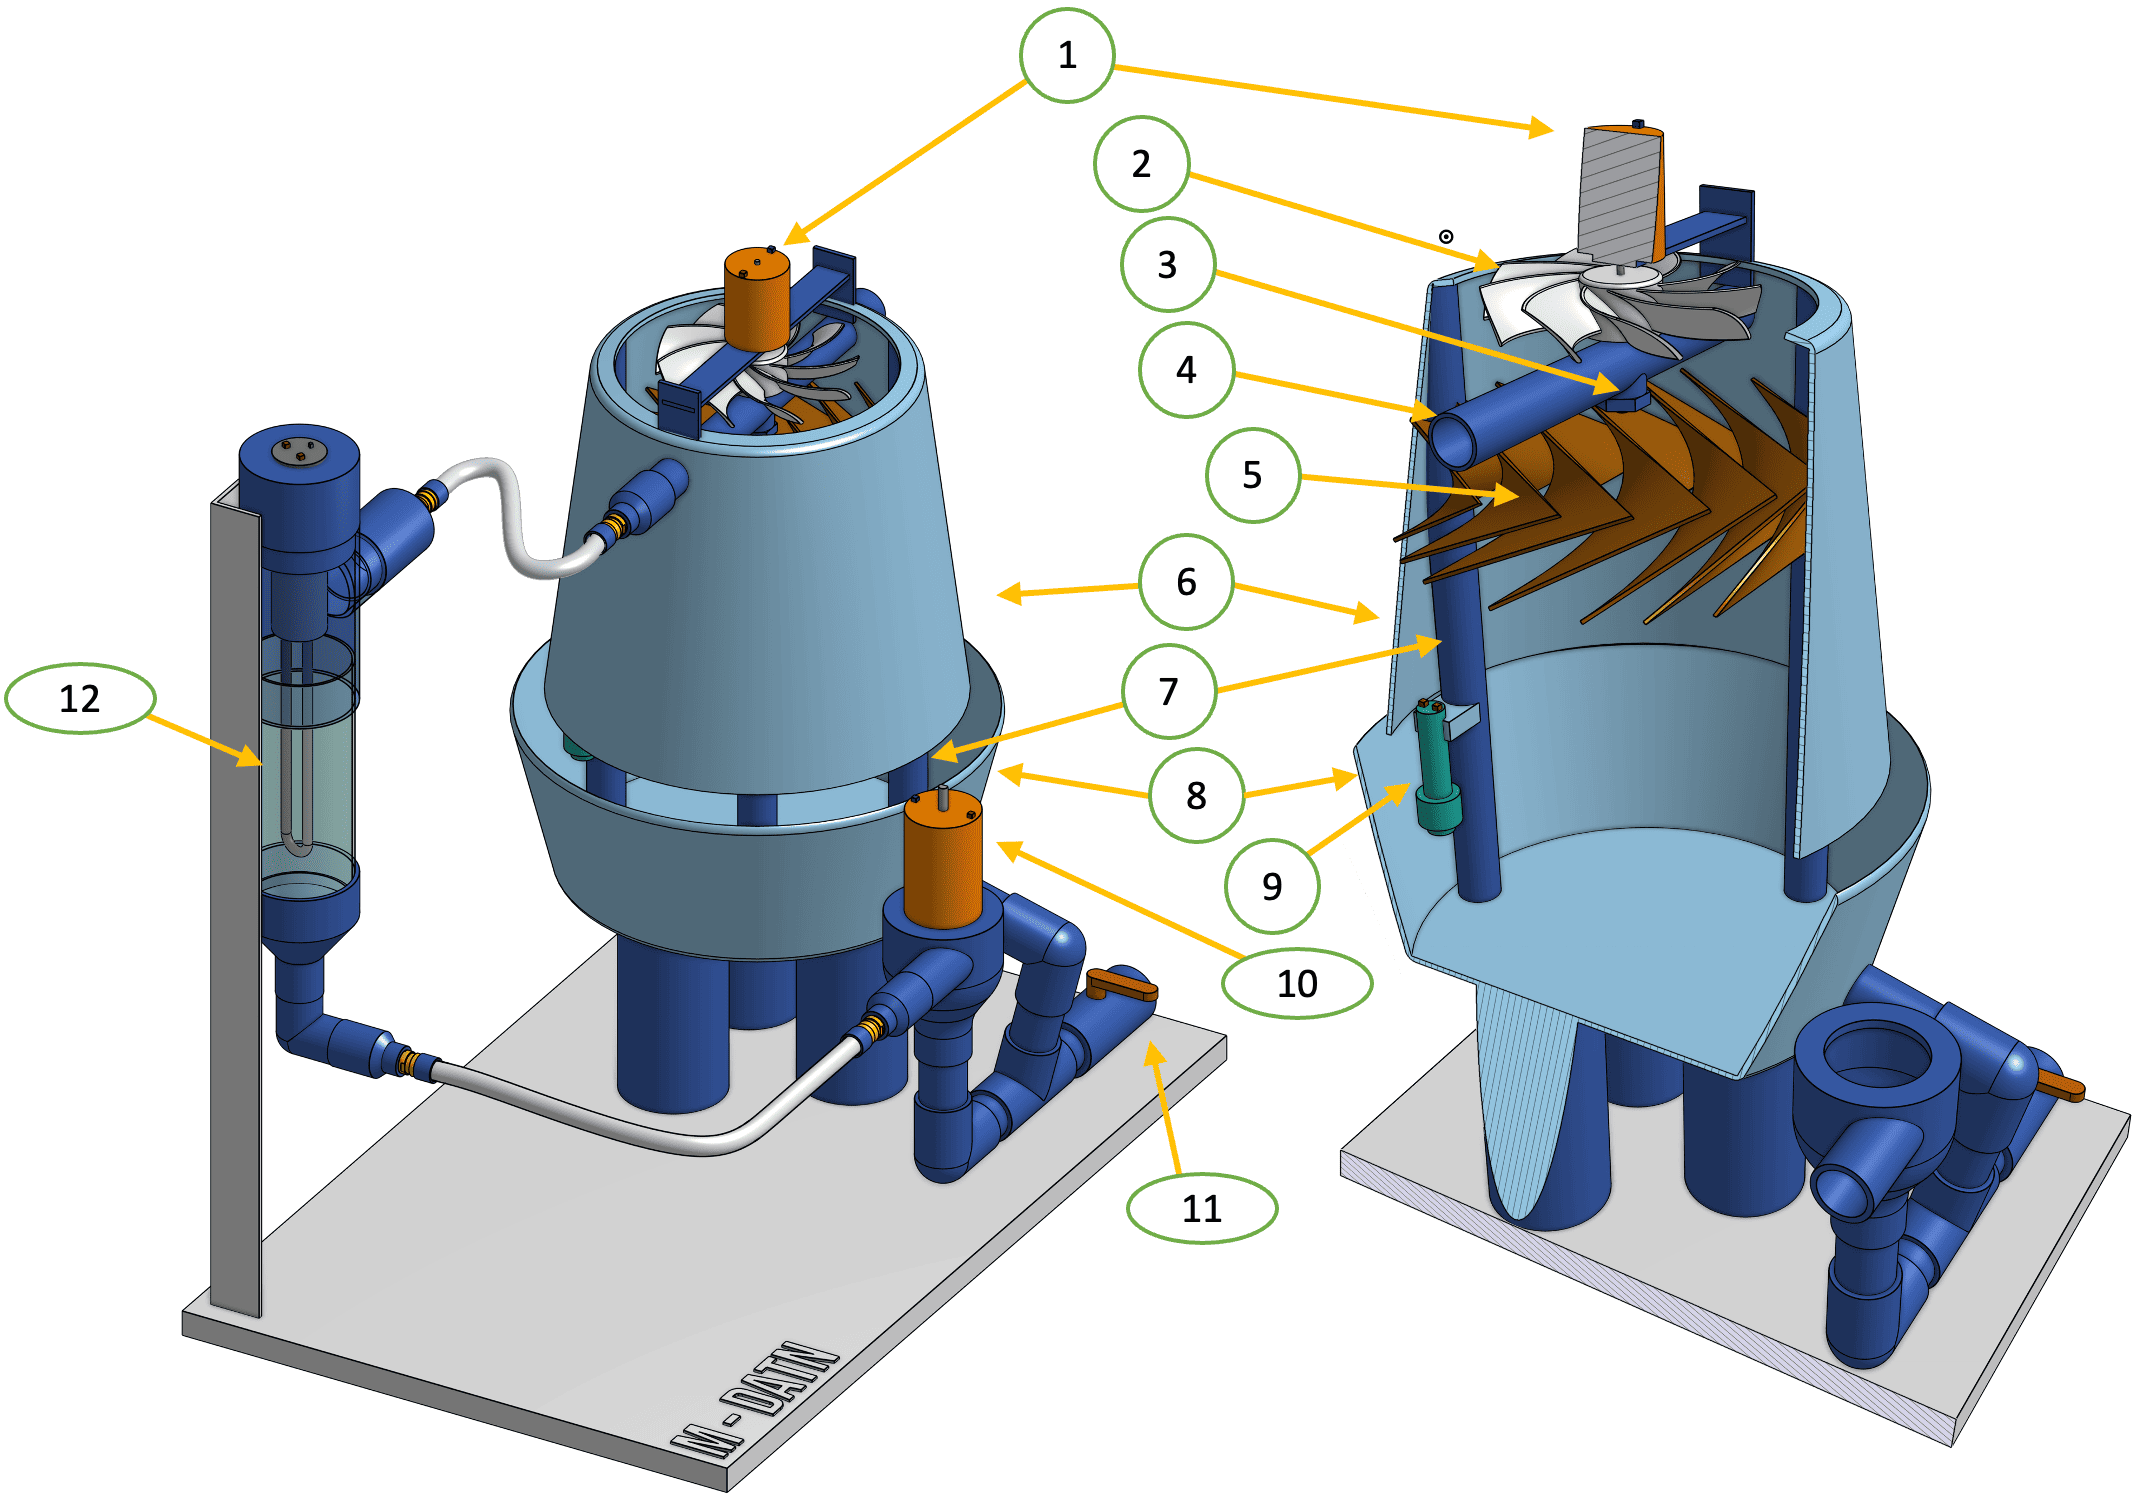
\includegraphics[width=1\textwidth]{Hinhve/chi_tiet_thap.png}
    \caption{Mô hình tháp giải nhiệt mini. (1- động cơ quạt; 2- cánh quạt hút; 3- vòi phun nước; 4- ống dẫn nước vào; 5- tấm phân phối nước; 6-thân tháp; 7- trụ đỡ thân tháp; 8- đáy tháp; 9- rơ le mức nước; 10- động cơ bơm; 11- van xả đáy; 12- tải nhiệt)}
    \label{fig:chi_tiet_thap}
\end{figure}

\subsection{Yêu cầu chức năng của hệ thống}
\label{sec:functional_requirements}

Hệ thống giám sát được thiết kế để đáp ứng các yêu cầu chức năng cơ bản sau:

\textbf{Thu thập dữ liệu thời gian thực:} Hệ thống phải có khả năng đo lường liên tục và chính xác các thông số vận hành với chu kỳ sampling phù hợp (30-60 giây), đảm bảo phát hiện kịp thời các thay đổi trong quá trình vận hành. Dữ liệu thu thập bao gồm nhiệt độ nước vào/ra với độ chính xác ±0,5°C, lưu lượng nước tuần hoàn với sai số ±10\%, và các thông số khí hậu xung quanh.

\textbf{Xử lý và tính toán tự động:} Hệ thống cần thực hiện tính toán thời gian thực các chỉ số hiệu suất phức tạp như công suất làm mát theo phương trình cân bằng năng lượng, hiệu suất tháp giải nhiệt dựa trên approach temperature, và nhiệt độ bầu ướt theo công thức Stull. Các tính toán này phải được thực hiện tự động mà không cần can thiệp thủ công.

\textbf{Lưu trữ và truy xuất dữ liệu:} Hệ thống phải có khả năng lưu trữ dữ liệu dài hạn trong cơ sở dữ liệu time-series, hỗ trợ truy vấn lịch sử và phân tích xu hướng. Dữ liệu cần được tổ chức có cấu trúc để thuận tiện cho việc xuất báo cáo và phân tích thống kê.

\textbf{Hiển thị và cảnh báo:} Hệ thống cung cấp giao diện trực quan hiển thị thông tin real-time, biểu đồ xu hướng và cơ chế cảnh báo tự động khi các thông số vượt ngưỡng định trước hoặc xuất hiện dấu hiệu bất thường.

\subsection{Yêu cầu kỹ thuật và vận hành}
\label{sec:technical_requirements}

\textbf{Độ chính xác và tin cậy:} Hệ thống phải đảm bảo độ chính xác đo lường phù hợp với yêu cầu đánh giá hiệu suất tháp giải nhiệt. Sai số tổng hợp trong tính toán công suất làm mát không vượt quá $\pm 5\%$, đáp ứng tiêu chuẩn ngành cho các ứng dụng giám sát năng lượng \cite{ashrae2020cooling}.

\textbf{Khả năng hoạt động liên tục:} Hệ thống được thiết kế để vận hành 24/7 trong môi trường có độ ẩm cao và nhiệt độ biến đổi. Thiết bị phải có khả năng tự phục hồi sau sự cố mạng hoặc mất điện tạm thời, với cơ chế lưu trữ dữ liệu cục bộ khi mất kết nối.

\textbf{Tính mở rộng và tích hợp:} Kiến trúc hệ thống cho phép mở rộng để giám sát nhiều tháp giải nhiệt hoặc tích hợp với các hệ thống quản lý năng lượng hiện có. Giao thức truyền thông sử dụng các tiêu chuẩn mở như MQTT và RESTful API.

\textbf{Chi phí triển khai hợp lý:} Giải pháp được tối ưu hóa chi phí thông qua việc sử dụng các thành phần phần cứng và phần mềm mã nguồn mở, với mục tiêu tổng chi phí đầu tư dưới 2 triệu VNĐ cho một đơn vị giám sát, phù hợp với khả năng đầu tư của doanh nghiệp vừa và nhỏ.

\section{Thiết kế và xây dựng hệ thống giám sát}
\label{sec:system_design_implementation_detail}

\subsection{Kiến trúc tổng thể hệ thống}
\label{sec:system_overview}

Dựa trên các yêu cầu chức năng và kỹ thuật đã xác định, hệ thống giám sát được thiết kế theo kiến trúc IoT phân tầng với năm lớp chức năng độc lập nhưng tương tác chặt chẽ. Kiến trúc này đảm bảo tính mô-đun, khả năng bảo trì và mở rộng, đồng thời tối ưu hóa hiệu suất xử lý và truyền thông.

\begin{figure}[H]
    \centering
    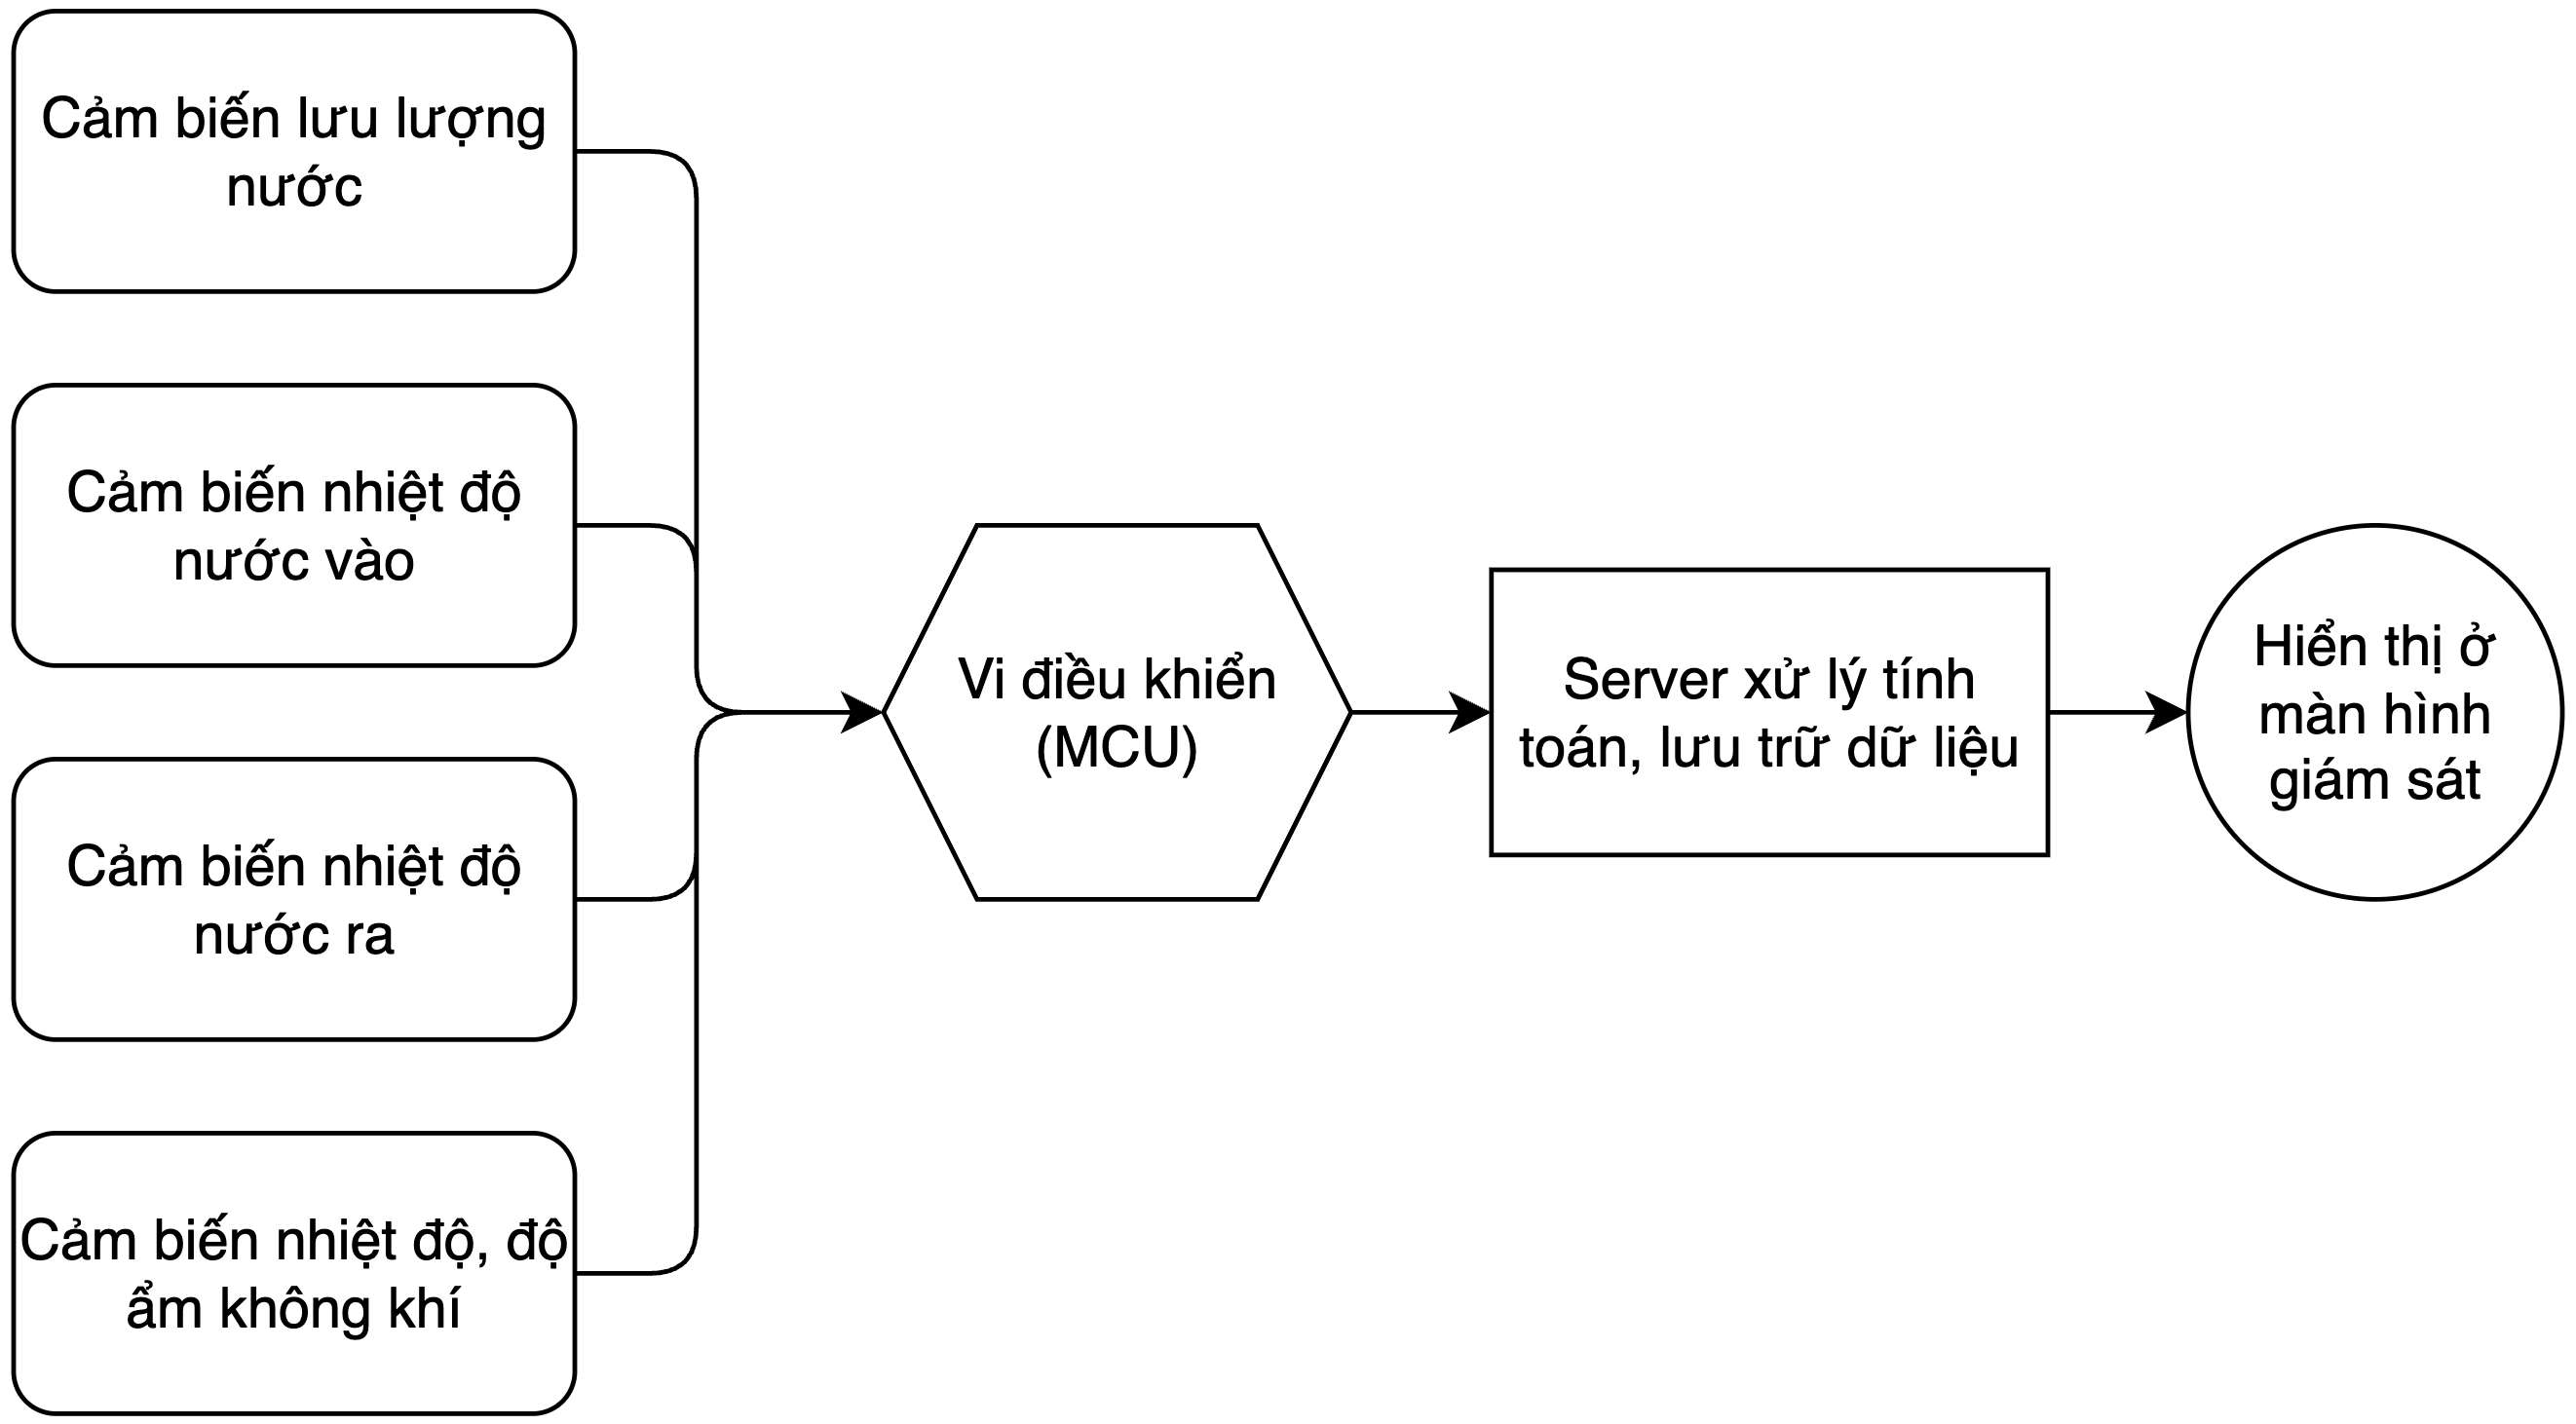
\includegraphics[width=0.95\textwidth]{../Hinhve/so_do_tong_quan_he_thong.png}
    \caption{Sơ đồ kiến trúc tổng thể hệ thống}
    \label{fig:system_diagram}
\end{figure}

\textbf{Lớp cảm biến} thực hiện thu thập dữ liệu đa tham số từ mô hình tháp giải nhiệt. Lớp này bao gồm mạng lưới cảm biến được phân bố tại các vị trí chiến lược để đo lường nhiệt độ nước vào/ra, lưu lượng tuần hoàn và điều kiện khí hậu xung quanh. Thiết kế đảm bảo độ chính xác và độ tin cậy cần thiết cho việc tính toán các chỉ số hiệu suất.

\textbf{Lớp điều khiển} sử dụng vi điều khiển ESP32 làm đơn vị xử lý edge computing, thực hiện thu thập dữ liệu đồng thời từ mạng cảm biến, xử lý sơ bộ và điều phối truyền tải. Kiến trúc dual-core cho phép xử lý song song các tác vụ thu thập dữ liệu và truyền thông mạng.

\textbf{Lớp truyền thông} triển khai giao thức MQTT over Wi-Fi với mã hóa TLS, đảm bảo truyền tải dữ liệu hiệu quả và bảo mật. Mô hình publish/subscribe cung cấp tính linh hoạt và khả năng mở rộng cho việc tích hợp nhiều thiết bị giám sát.

\textbf{Lớp xử lý dữ liệu} bao gồm hệ thống backend thực hiện các tính toán phức tạp vượt khả năng vi điều khiển, bao gồm tính toán nhiệt độ bầu ướt, công suất làm mát và các chỉ số hiệu suất. Dữ liệu được lưu trữ trong cơ sở dữ liệu time-series để hỗ trợ phân tích xu hướng.

\textbf{Lớp giao diện người dùng} cung cấp dashboard trực quan với các chức năng hiển thị real-time, phân tích xu hướng và cảnh báo tự động. Giao diện được tối ưu cho trải nghiệm người dùng và hỗ trợ ra quyết định vận hành.

\subsection{Nguyên lý hoạt động của hệ thống}
\label{sec:system_operation_principle}

Hệ thống giám sát hoạt động theo chu trình liên tục với các giai đoạn xử lý được tối ưu để đảm bảo độ chính xác và tính kịp thời của thông tin. ESP32 thực hiện thu thập dữ liệu từ các cảm biến nhiệt độ, độ ẩm và lưu lượng nước theo chu kỳ tối ưu, cân bằng giữa độ chính xác dữ liệu và hiệu quả sử dụng tài nguyên hệ thống.

Vi điều khiển thực hiện xử lý sơ bộ bao gồm kiểm tra tính hợp lệ dữ liệu, loại bỏ nhiễu và tính toán các thông số cơ bản. Xử lý tại chỗ giúp giảm tải cho hệ thống backend và đảm bảo chỉ dữ liệu chất lượng cao được truyền đi.

Dữ liệu sau xử lý được đóng gói định dạng JSON và truyền tải lên MQTT Broker qua kết nối Wi-Fi được bảo vệ bằng mã hóa TLS. Giao thức MQTT đảm bảo truyền tải hiệu quả trong điều kiện băng thông hạn chế, cung cấp các cơ chế tin cậy như Quality of Service phân cấp và duy trì phiên làm việc.

Hệ thống backend tiếp nhận dữ liệu từ MQTT Broker và thực hiện các tính toán phức tạp bao gồm tính toán nhiệt độ bầu ướt theo công thức Stull, xác định công suất làm mát dựa trên lưu lượng và chênh lệch nhiệt độ, cũng như đánh giá hiệu suất làm mát của tháp giải nhiệt. Các tính toán này yêu cầu tài nguyên xử lý đáng kể và được thực hiện tập trung để tối ưu hiệu suất.

Toàn bộ dữ liệu được lưu trữ có hệ thống trong cơ sở dữ liệu time-series chuyên biệt, hỗ trợ phân tích xu hướng dài hạn và truy vấn dữ liệu lịch sử phức tạp. Dữ liệu được hiển thị trên dashboard trực quan cho phép kỹ sư vận hành giám sát tình trạng hệ thống chi tiết theo thời gian thực. Hệ thống tích hợp các module giám sát thông minh và cảnh báo tự động, có khả năng phát hiện sớm dấu hiệu bất thường và thông báo kịp thời khi thông số vượt ngưỡng an toàn hoặc xuất hiện xu hướng suy giảm hiệu suất.

\section{Lựa chọn phần cứng}
\label{sec:hardware_selection}

Lựa chọn phần cứng cho hệ thống giám sát tháp giải nhiệt đáp ứng các yêu cầu kỹ thuật cụ thể và điều kiện vận hành đặc thù. Hệ thống thu thập đồng thời các thông số nhiệt độ nước vào/ra, nhiệt độ và độ ẩm không khí xung quanh, cùng lưu lượng nước tuần hoàn. Việc lựa chọn thiết bị đảm bảo khả năng xử lý dữ liệu cục bộ và truyền thông real-time trong môi trường có độ ẩm cao và hóa chất xử lý nước. Các tiêu chí thiết kế tuân thủ khuyến nghị trong sổ tay thực hành HVAC và hướng dẫn vận hành tháp giải nhiệt \cite{ashrae2020cooling,epa_cooling_tower_guide_2017}.

\subsection{Vi điều khiển ESP32}
\label{sec:esp32_controller}

Vi điều khiển ESP32 được lựa chọn làm đơn vị xử lý trung tâm nhờ năng lực tính toán phù hợp, kết nối mạng tích hợp và hiệu quả kinh tế \cite{Espressif_ESP32_technical_reference}. ESP32 sử dụng kiến trúc dual-core 32-bit Xtensa LX6 với xung nhịp tối đa 240\,MHz, đủ khả năng thực hiện song song các tác vụ edge computing như thu thập dữ liệu đa cảm biến, lọc/tiền xử lý và đóng gói truyền thông.

\begin{figure}[H]
    \centering
    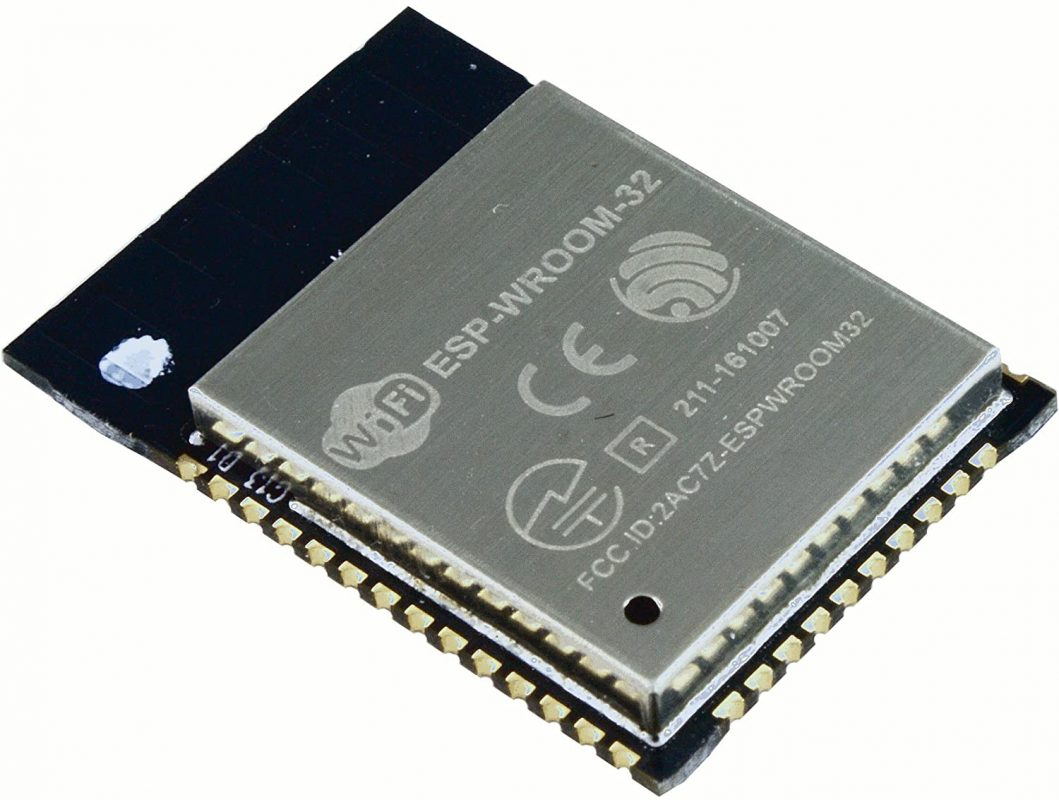
\includegraphics[width=0.5\textwidth]{../Hinhve/ESP32-WROOM-32-1059x800.jpg}
    \caption{Vi điều khiển ESP32-WROOM-32 \cite{Espressif_ESP32_technical_reference}}
    \label{fig:esp32}
\end{figure}

Thiết bị tích hợp WiFi 802.11 b/g/n và Bluetooth v4.2, loại bỏ nhu cầu module mạng rời và giảm độ phức tạp phần cứng. Hệ ngoại vi bao gồm SPI, I\textsuperscript{2}C, UART, PWM, ADC SAR 12-bit và DAC 8-bit, cho phép giao tiếp trực tiếp với đa số cảm biến\footnote{Giao tiếp 1-Wire với DS18B20 được thực hiện bằng phần mềm (bit-banging).}. Cơ chế quản lý năng lượng hỗ trợ các chế độ tiết kiệm bao gồm deep-sleep với dòng tiêu thụ từ vài đến vài chục microampere, phù hợp cho vận hành liên tục với chi phí năng lượng thấp \cite{Espressif_ESP32_technical_reference}.

ESP32 cân bằng tối ưu giữa năng lực xử lý, kết nối không dây tích hợp và chi phí triển khai. Hệ sinh thái phần mềm phong phú với Arduino IDE, ESP-IDF và MicroPython tạo thuận lợi cho phát triển và bảo trì hệ thống IoT giám sát real-time \cite{Espressif_ESP32_technical_reference}.

\subsection{Cảm biến nhiệt độ DS18B20}
\label{sec:ds18b20_sensor}

Cảm biến nhiệt độ số DS18B20 được sử dụng để đo nhiệt độ nước tại điểm vào và ra của tháp giải nhiệt. Thiết bị có độ chính xác $\pm 0.5^\circ\mathrm{C}$ trong dải vận hành $-10^\circ\mathrm{C}$ đến $+85^\circ\mathrm{C}$, dải đo mở rộng từ $-55^\circ\mathrm{C}$ đến $+125^\circ\mathrm{C}$ với độ phân giải cấu hình được từ 9 đến 12 bit. Cảm biến hoạt động với nguồn 3.0-5.5 V và hỗ trợ chế độ parasitic power để giảm thiểu số dây dẫn \cite{datasheet_DS18B20}. Việc sử dụng hai cảm biến cùng loại đảm bảo tính nhất quán phép đo và thuận lợi cho tính toán chênh lệch nhiệt độ $\Delta T$ phục vụ cân bằng năng lượng.

\begin{figure}[H]
    \centering
    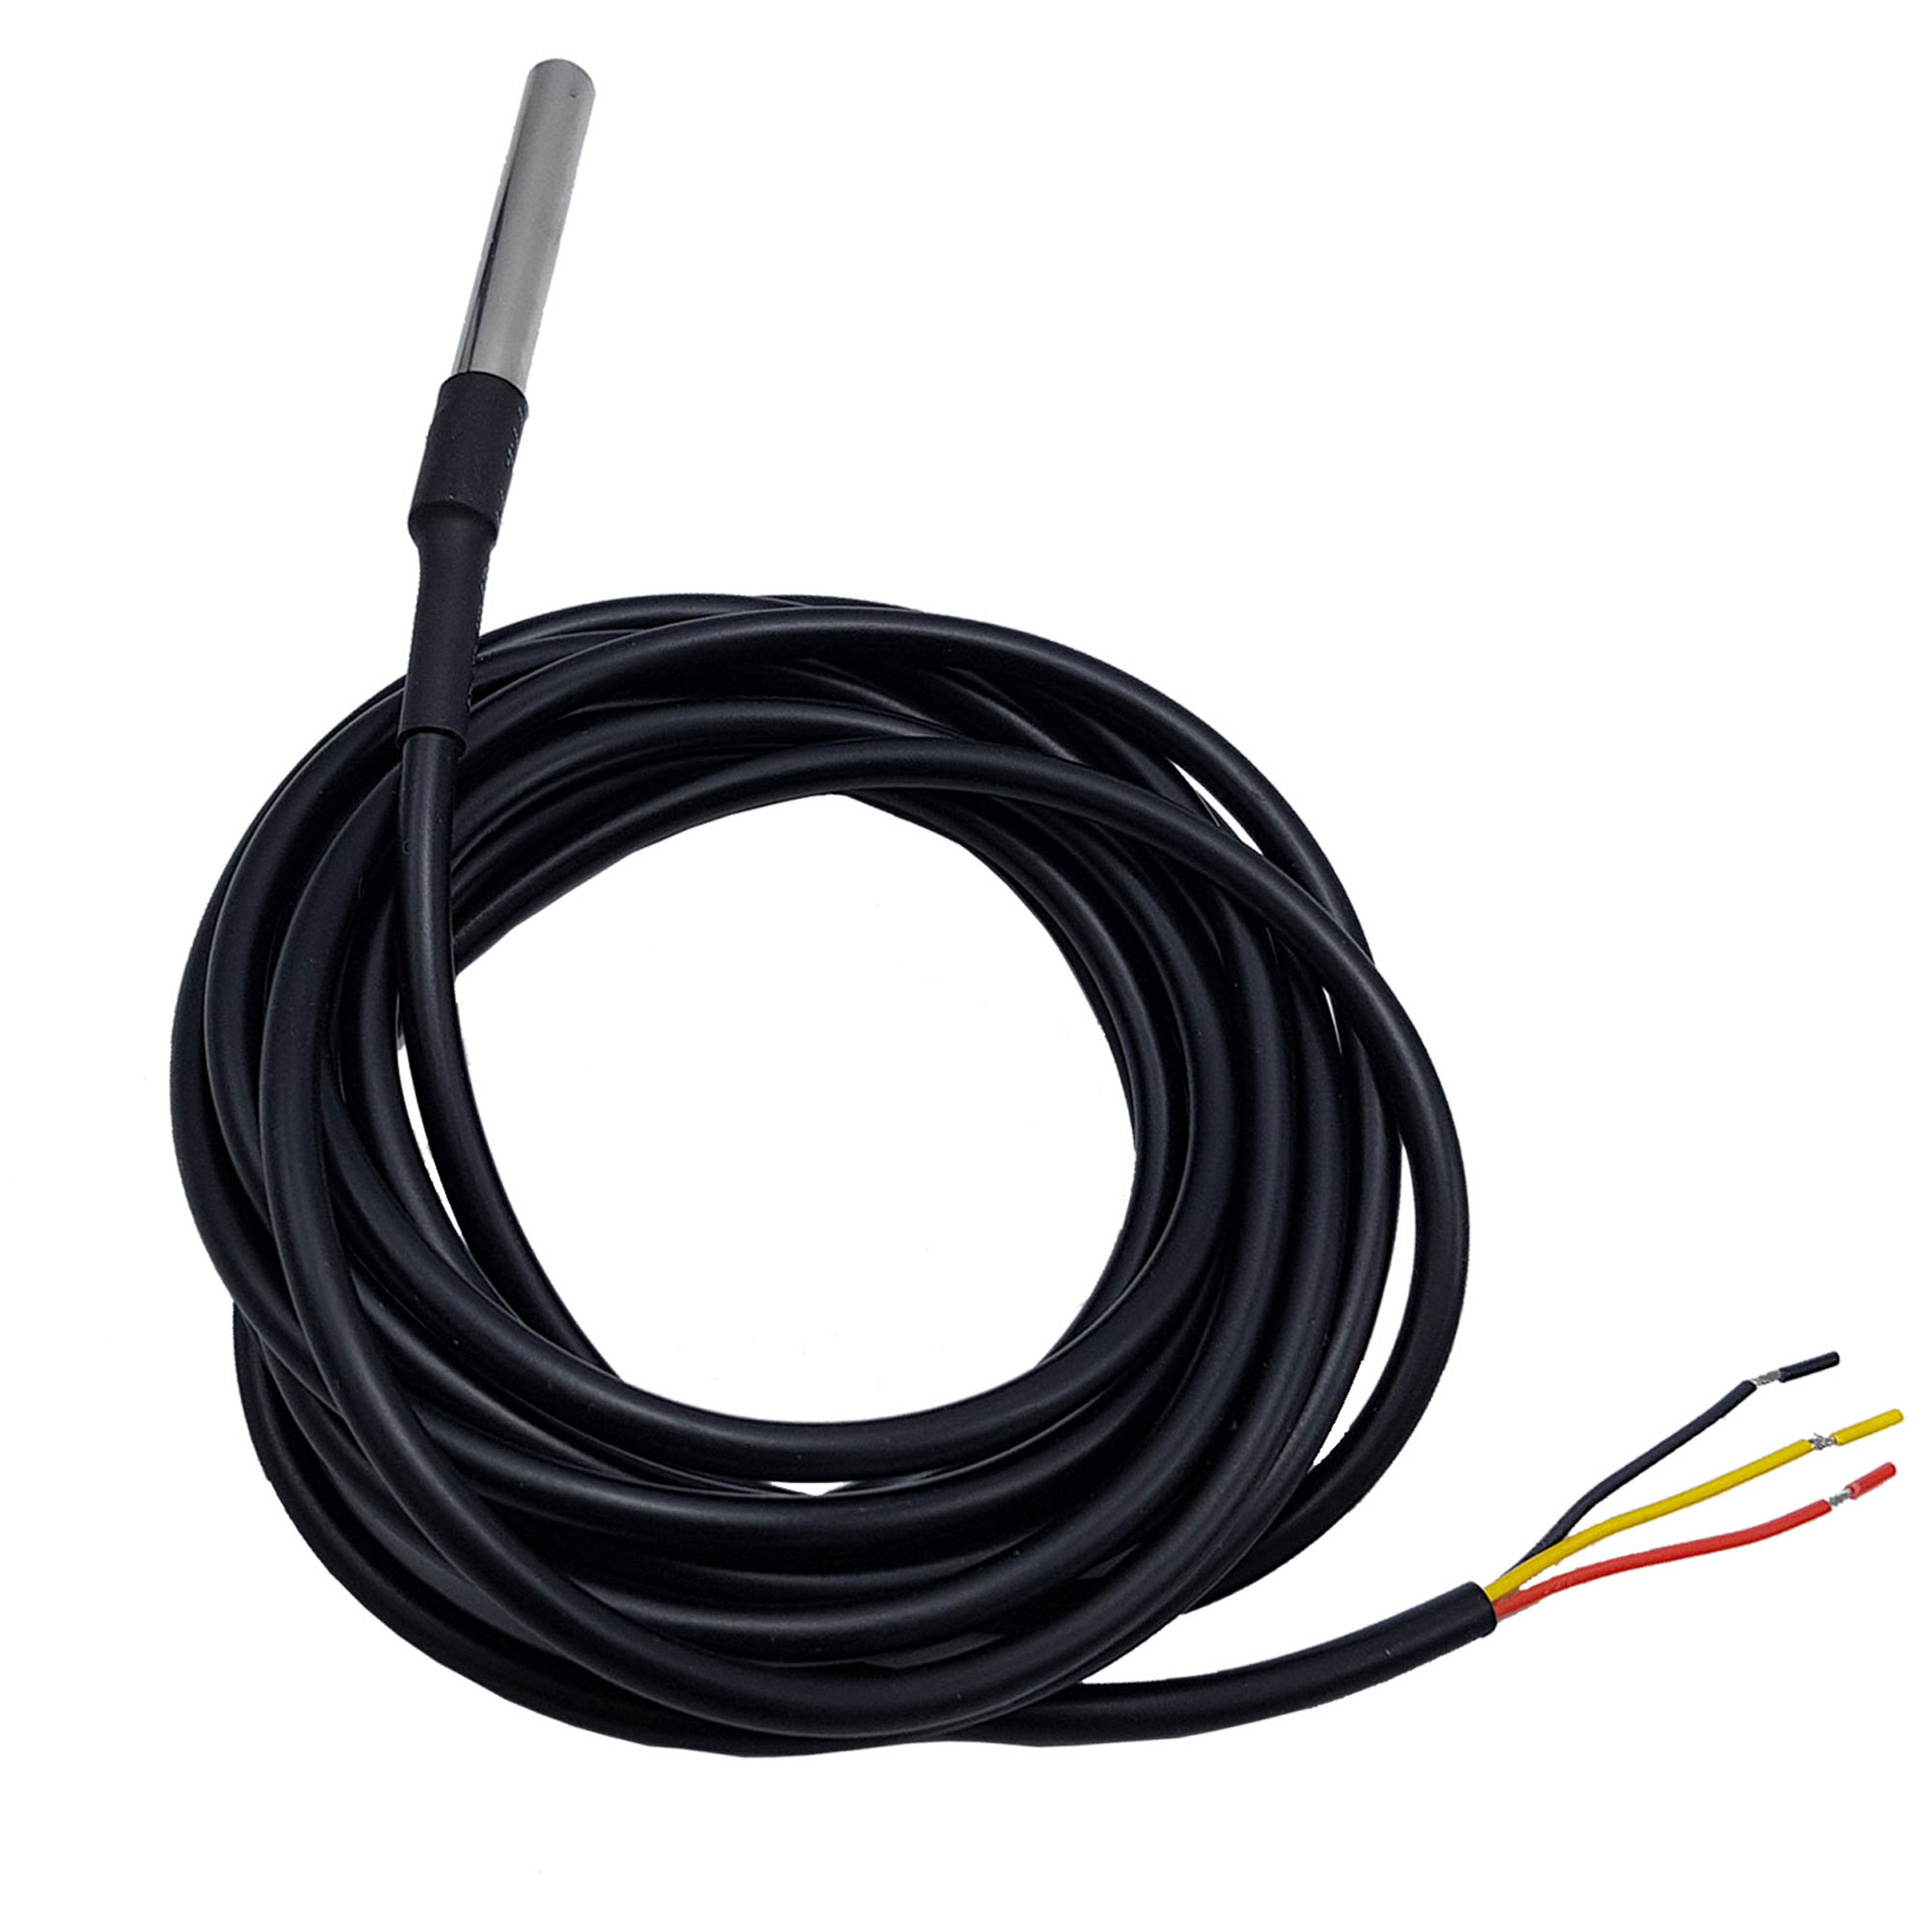
\includegraphics[width=0.5\textwidth]{../Hinhve/DS18B20.jpg}
    \caption{Cảm biến nhiệt độ DS18B20 \cite{datasheet_DS18B20}}
    \label{fig:ds18b20}
\end{figure}

DS18B20 được lựa chọn nhờ sai số đo lường $\pm 0.5^\circ\mathrm{C}$ đáp ứng yêu cầu độ chính xác cho tính toán công suất làm mát. Giao thức 1-Wire cho phép kết nối nhiều cảm biến trên cùng đường tín hiệu, giảm độ phức tạp thiết kế mạch và hệ thống dây dẫn \cite{datasheet_DS18B20}.

\subsection{Cảm biến độ ẩm và nhiệt độ DHT22}
\label{sec:dht22_sensor}

\begin{figure}[H]
    \centering
    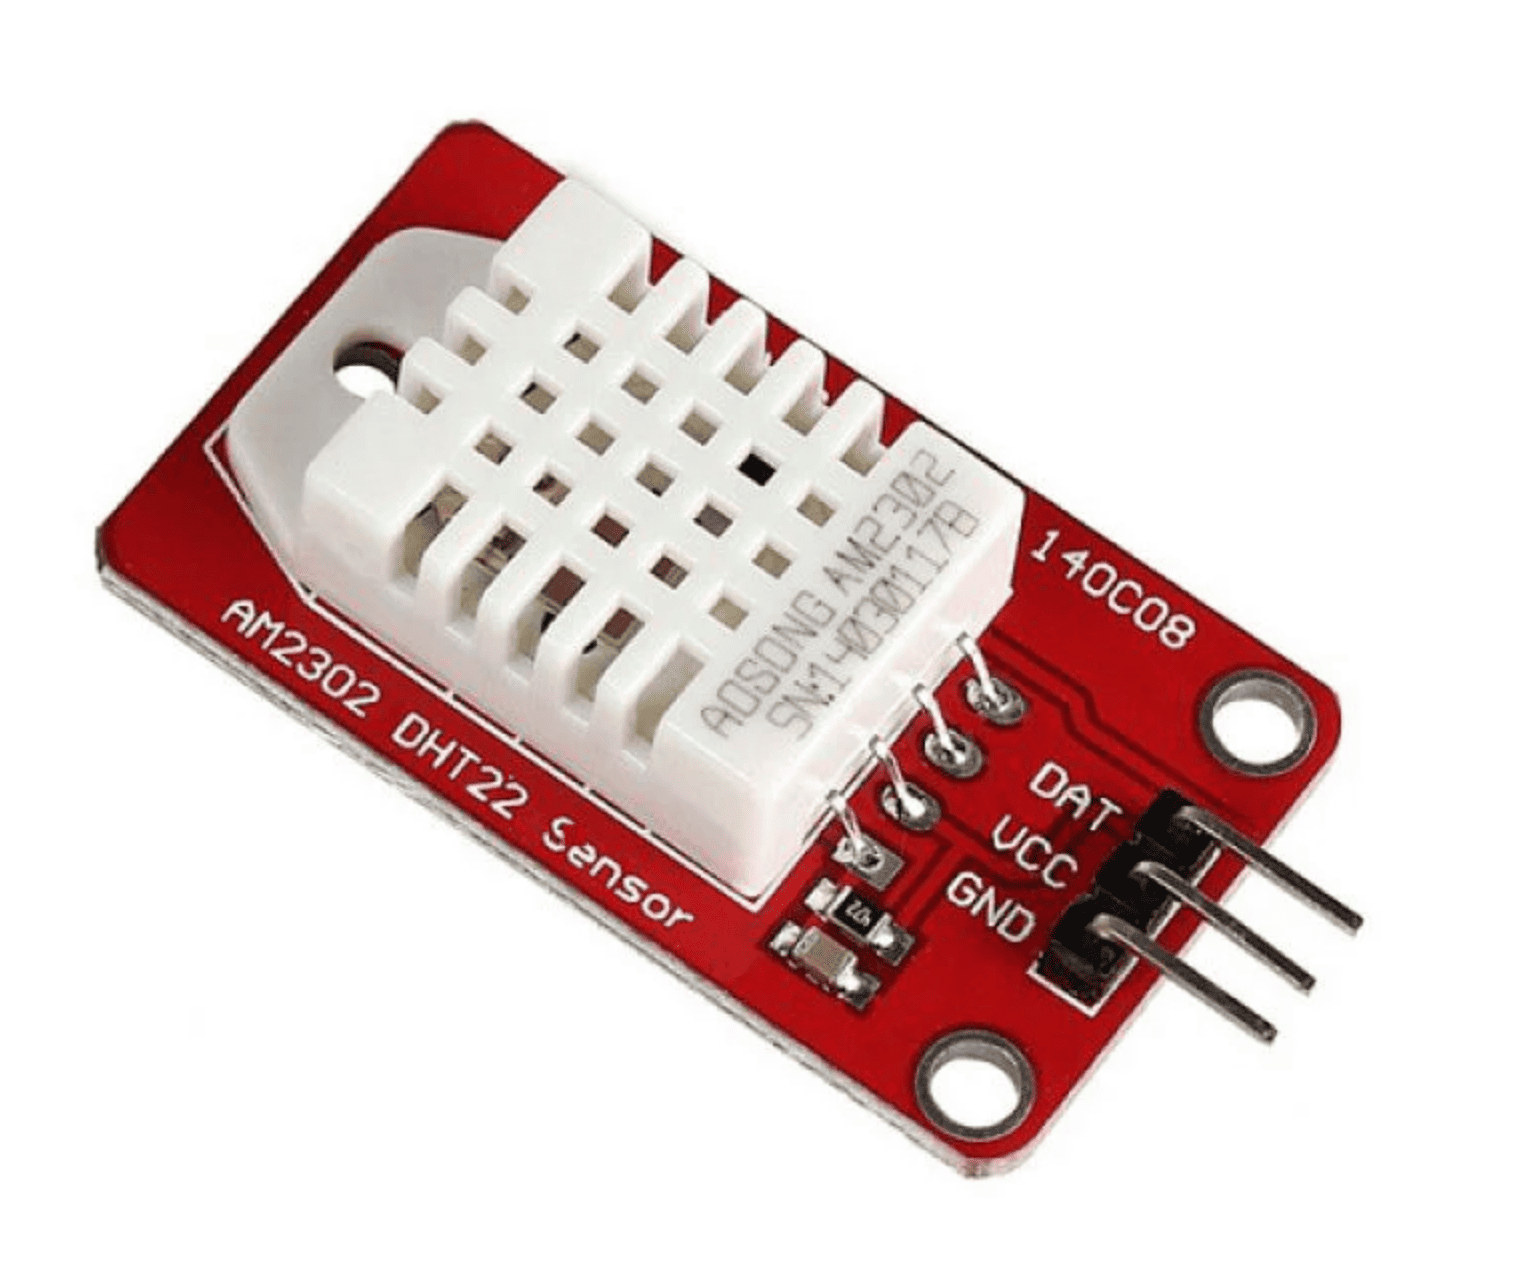
\includegraphics[width=0.5\textwidth]{../Hinhve/DHT22.png}
    \caption{Cảm biến nhiệt độ/độ ẩm DHT22 \cite{datasheet_DHT22}}
    \label{fig:dht22}
\end{figure}

Cảm biến DHT22 (AM2302) đo lường đồng thời nhiệt độ và độ ẩm tương đối không khí xung quanh tháp giải nhiệt. Dữ liệu thu được làm đầu vào cho ước tính nhiệt độ bầu ướt theo công thức Stull \cite{datasheet_DHT22,stull2011meteorology}. Thiết bị có độ chính xác nhiệt độ $\pm 0.5^\circ\mathrm{C}$ trong dải $-40^\circ\mathrm{C}$ đến $+80^\circ\mathrm{C}$ và độ chính xác độ ẩm $\pm 2\%$ RH (tối đa $\pm 5\%$) trong dải 0-100\% RH. Độ phân giải đạt 0.1 với chu kỳ sampling tối thiểu 2 giây. Giao thức truyền thông single-wire proprietary (khác với chuẩn 1-Wire) đơn giản hóa kết nối với vi điều khiển \cite{datasheet_DHT22}.

DHT22 được lựa chọn nhờ cân bằng hiệu quả giữa chi phí và độ chính xác đo lường nhiệt độ-độ ẩm không khí. Độ chính xác thiết bị đáp ứng yêu cầu ước tính nhiệt độ bầu ướt $T_\mathrm{wb}$ và đánh giá hiệu suất bay hơi của tháp giải nhiệt \cite{datasheet_DHT22,stull2011meteorology}.

\subsection{Cảm biến lưu lượng nước YF-S201}
\label{sec:yf_s201_sensor}

Cảm biến lưu lượng YF-S201 được sử dụng để đo lưu lượng nước tuần hoàn trong hệ thống tháp giải nhiệt\footnote{Trong hệ thống công nghiệp thực tế, các lưu lượng kế điện từ, siêu âm hoặc vortex thường được ưu tiên do độ chính xác và độ bền cao hơn \cite{ashrae2020cooling,epa_watersense_cooling_towers_2012}. YF-S201 được lựa chọn phù hợp với quy mô mô hình thí nghiệm.}. Thiết bị hoạt động theo nguyên lý turbine gắn nam châm kết hợp cảm biến Hall Effect. Khi cực từ di chuyển qua phần tử Hall, xung điện được tạo ra với tần số tỷ lệ thuận với lưu lượng thể tích \cite{datasheet_YFS201}.

Thông số kỹ thuật YF-S201 bao gồm dải đo 1-30 L/min, sai số điển hình $\pm 10\%$, áp suất làm việc tối đa 1.75 MPa và dải nhiệt độ 0-80°C. Thiết bị yêu cầu nguồn 5-18 V DC và cung cấp tín hiệu xung TTL 5 V. Hệ số chuyển đổi danh định khoảng 7.5 xung/giây cho mỗi L/min, giá trị thực tế phụ thuộc cấu hình đường ống và điều kiện lắp đặt, đòi hỏi hiệu chuẩn hiện trường \cite{datasheet_YFS201}.

\begin{figure}[H]
    \centering
    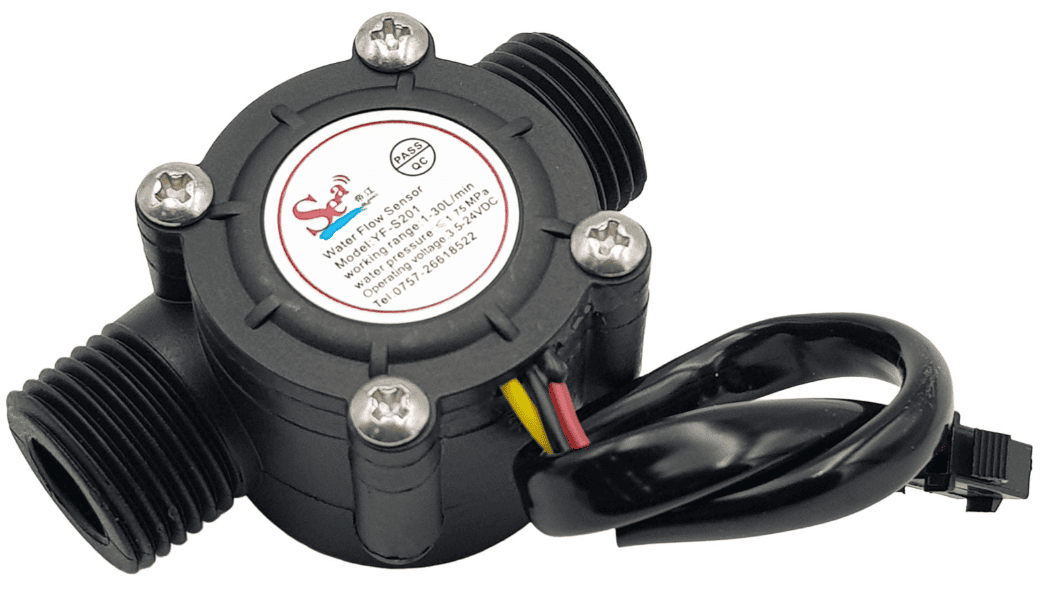
\includegraphics[width=0.5\textwidth]{../Hinhve/YF-S201.png}
    \caption{Cảm biến lưu lượng nước YF-S201 \cite{datasheet_YFS201}}
    \label{fig:yf-s201}
\end{figure}

YF-S201 được lựa chọn nhờ dải đo phù hợp quy mô mô hình thí nghiệm và tín hiệu xung TTL tương thích trực tiếp với ESP32. Thiết bị có chi phí thấp và lắp đặt đơn giản, phù hợp mục tiêu đồ án \cite{datasheet_YFS201}.

\subsection{Lưu ý lắp đặt và bảo vệ thiết bị}
\label{sec:installation_protection}

Môi trường vận hành tháp giải nhiệt đặc trưng bởi độ ẩm cao, dao động nhiệt độ và hóa chất xử lý như clo và chất diệt tảo, có thể ảnh hưởng tiêu cực đến độ tin cậy thiết bị điện tử. Để đảm bảo hoạt động ổn định, hệ thống cần vỏ bảo vệ tiêu chuẩn IP65 trở lên, vật liệu và đầu dò chống ăn mòn, hệ thống dây và nối đất đúng quy cách để hạn chế nhiễu điện từ, cùng quy trình hiệu chuẩn định kỳ cho cảm biến lưu lượng và nhiệt độ \cite{epa_cooling_tower_guide_2017,epa_watersense_cooling_towers_2012}.

\subsection{Thảo luận lựa chọn thiết bị}
\label{sec:device_selection_discussion}

Quá trình lựa chọn phần cứng dựa trên các tiêu chí: sự phù hợp dải đo và sai số với yêu cầu ứng dụng, độ bền trong điều kiện môi trường khắc nghiệt, khả năng tích hợp với hệ thống tổng thể và tối ưu chi phí sở hữu.

\subsubsection{So sánh vi điều khiển}
\label{sec:microcontroller_comparison}

So với các vi điều khiển 8-bit như Arduino Uno/ATmega328P, ESP32 có ưu thế vượt trội về năng lực xử lý và kết nối không dây tích hợp. Nền tảng 8-bit thiếu khả năng kết nối mạng và có tài nguyên xử lý hạn chế, trong khi ESP32 cung cấp WiFi/BLE tích hợp và giảm nhu cầu phần cứng phụ trợ \cite{Espressif_ESP32_technical_reference,microchip_atmega328p}. So với máy tính nhúng như Raspberry Pi 4, ESP32 có lợi thế về tiêu thụ năng lượng thấp, thời gian khởi động nhanh, cấu trúc cơ khí đơn giản và chi phí thấp, vẫn đáp ứng yêu cầu edge computing. Raspberry Pi 4 phù hợp hơn cho vai trò local server hoặc edge gateway \cite{raspberrypi4_specs}.

\subsubsection{So sánh cảm biến nhiệt độ}
\label{sec:temperature_sensor_comparison}

DS18B20 đáp ứng yêu cầu sai số đo lường và dễ tích hợp qua giao thức 1-Wire cho ứng dụng đo nhiệt độ nước. Các cảm biến RTD (PT100/PT1000) có độ chính xác và ổn định cao hơn nhưng yêu cầu mạch biến đổi tín hiệu phức tạp và hiệu chuẩn khắt khe. Cặp nhiệt có ưu điểm dải đo rộng và thời gian đáp ứng nhanh, nhưng cần bù nhiệt độ đầu lạnh và độ chính xác thấp hơn trong dải nhiệt độ ứng dụng \cite{datasheet_DS18B20,ashrae2020cooling}. Trong phạm vi mô hình thí nghiệm, DS18B20 là lựa chọn tối ưu cân bằng hiệu năng và chi phí.

\subsubsection{So sánh cảm biến độ ẩm}
\label{sec:humidity_sensor_comparison}

DHT22 cung cấp độ chính xác phù hợp cho ước tính nhiệt độ bầu ướt $T_\mathrm{wb}$ trong phạm vi ứng dụng này. Đối với môi trường công nghiệp khắc nghiệt hoặc yêu cầu sai số thấp hơn, có thể xem xét dòng cảm biến SHT3x như SHT35 với độ chính xác cao hơn ($\pm 1.5\%$ RH và $\pm 0.1^\circ\mathrm{C}$) và giao tiếp I\textsuperscript{2}C tiêu chuẩn \cite{sensirion_sht3x_dis}. Tuy nhiên, lựa chọn này cần cân nhắc yếu tố chi phí và độ phức tạp tích hợp hệ thống.

\subsubsection{So sánh cảm biến lưu lượng}
\label{sec:flow_sensor_comparison}

Các công nghệ đo lưu lượng phổ biến bao gồm turbine cơ học (YF-S201), điện từ và siêu âm. Trong quy mô mô hình thí nghiệm, cảm biến turbine đáp ứng yêu cầu theo dõi xu hướng và ước lượng lưu lượng với chi phí hợp lý, tuy cần hiệu chuẩn hiện trường và chú ý lắng cặn cùng hàm lượng chất rắn trong nước. Đối với quy mô công nghiệp, lưu lượng kế điện từ (không có bộ phận chuyển động, độ chính xác cao) hoặc siêu âm (inline/clamp-on, không xâm nhập) thường được ưu tiên do độ bền và độ chính xác cao, mặc dù đòi hỏi chi phí lớn hơn và điều kiện lắp đặt khắt khe \cite{ashrae2020cooling,epa_watersense_cooling_towers_2012}.

\subsubsection{Kết luận lựa chọn}
\label{sec:selection_conclusion}

\begin{figure}
    \centering
    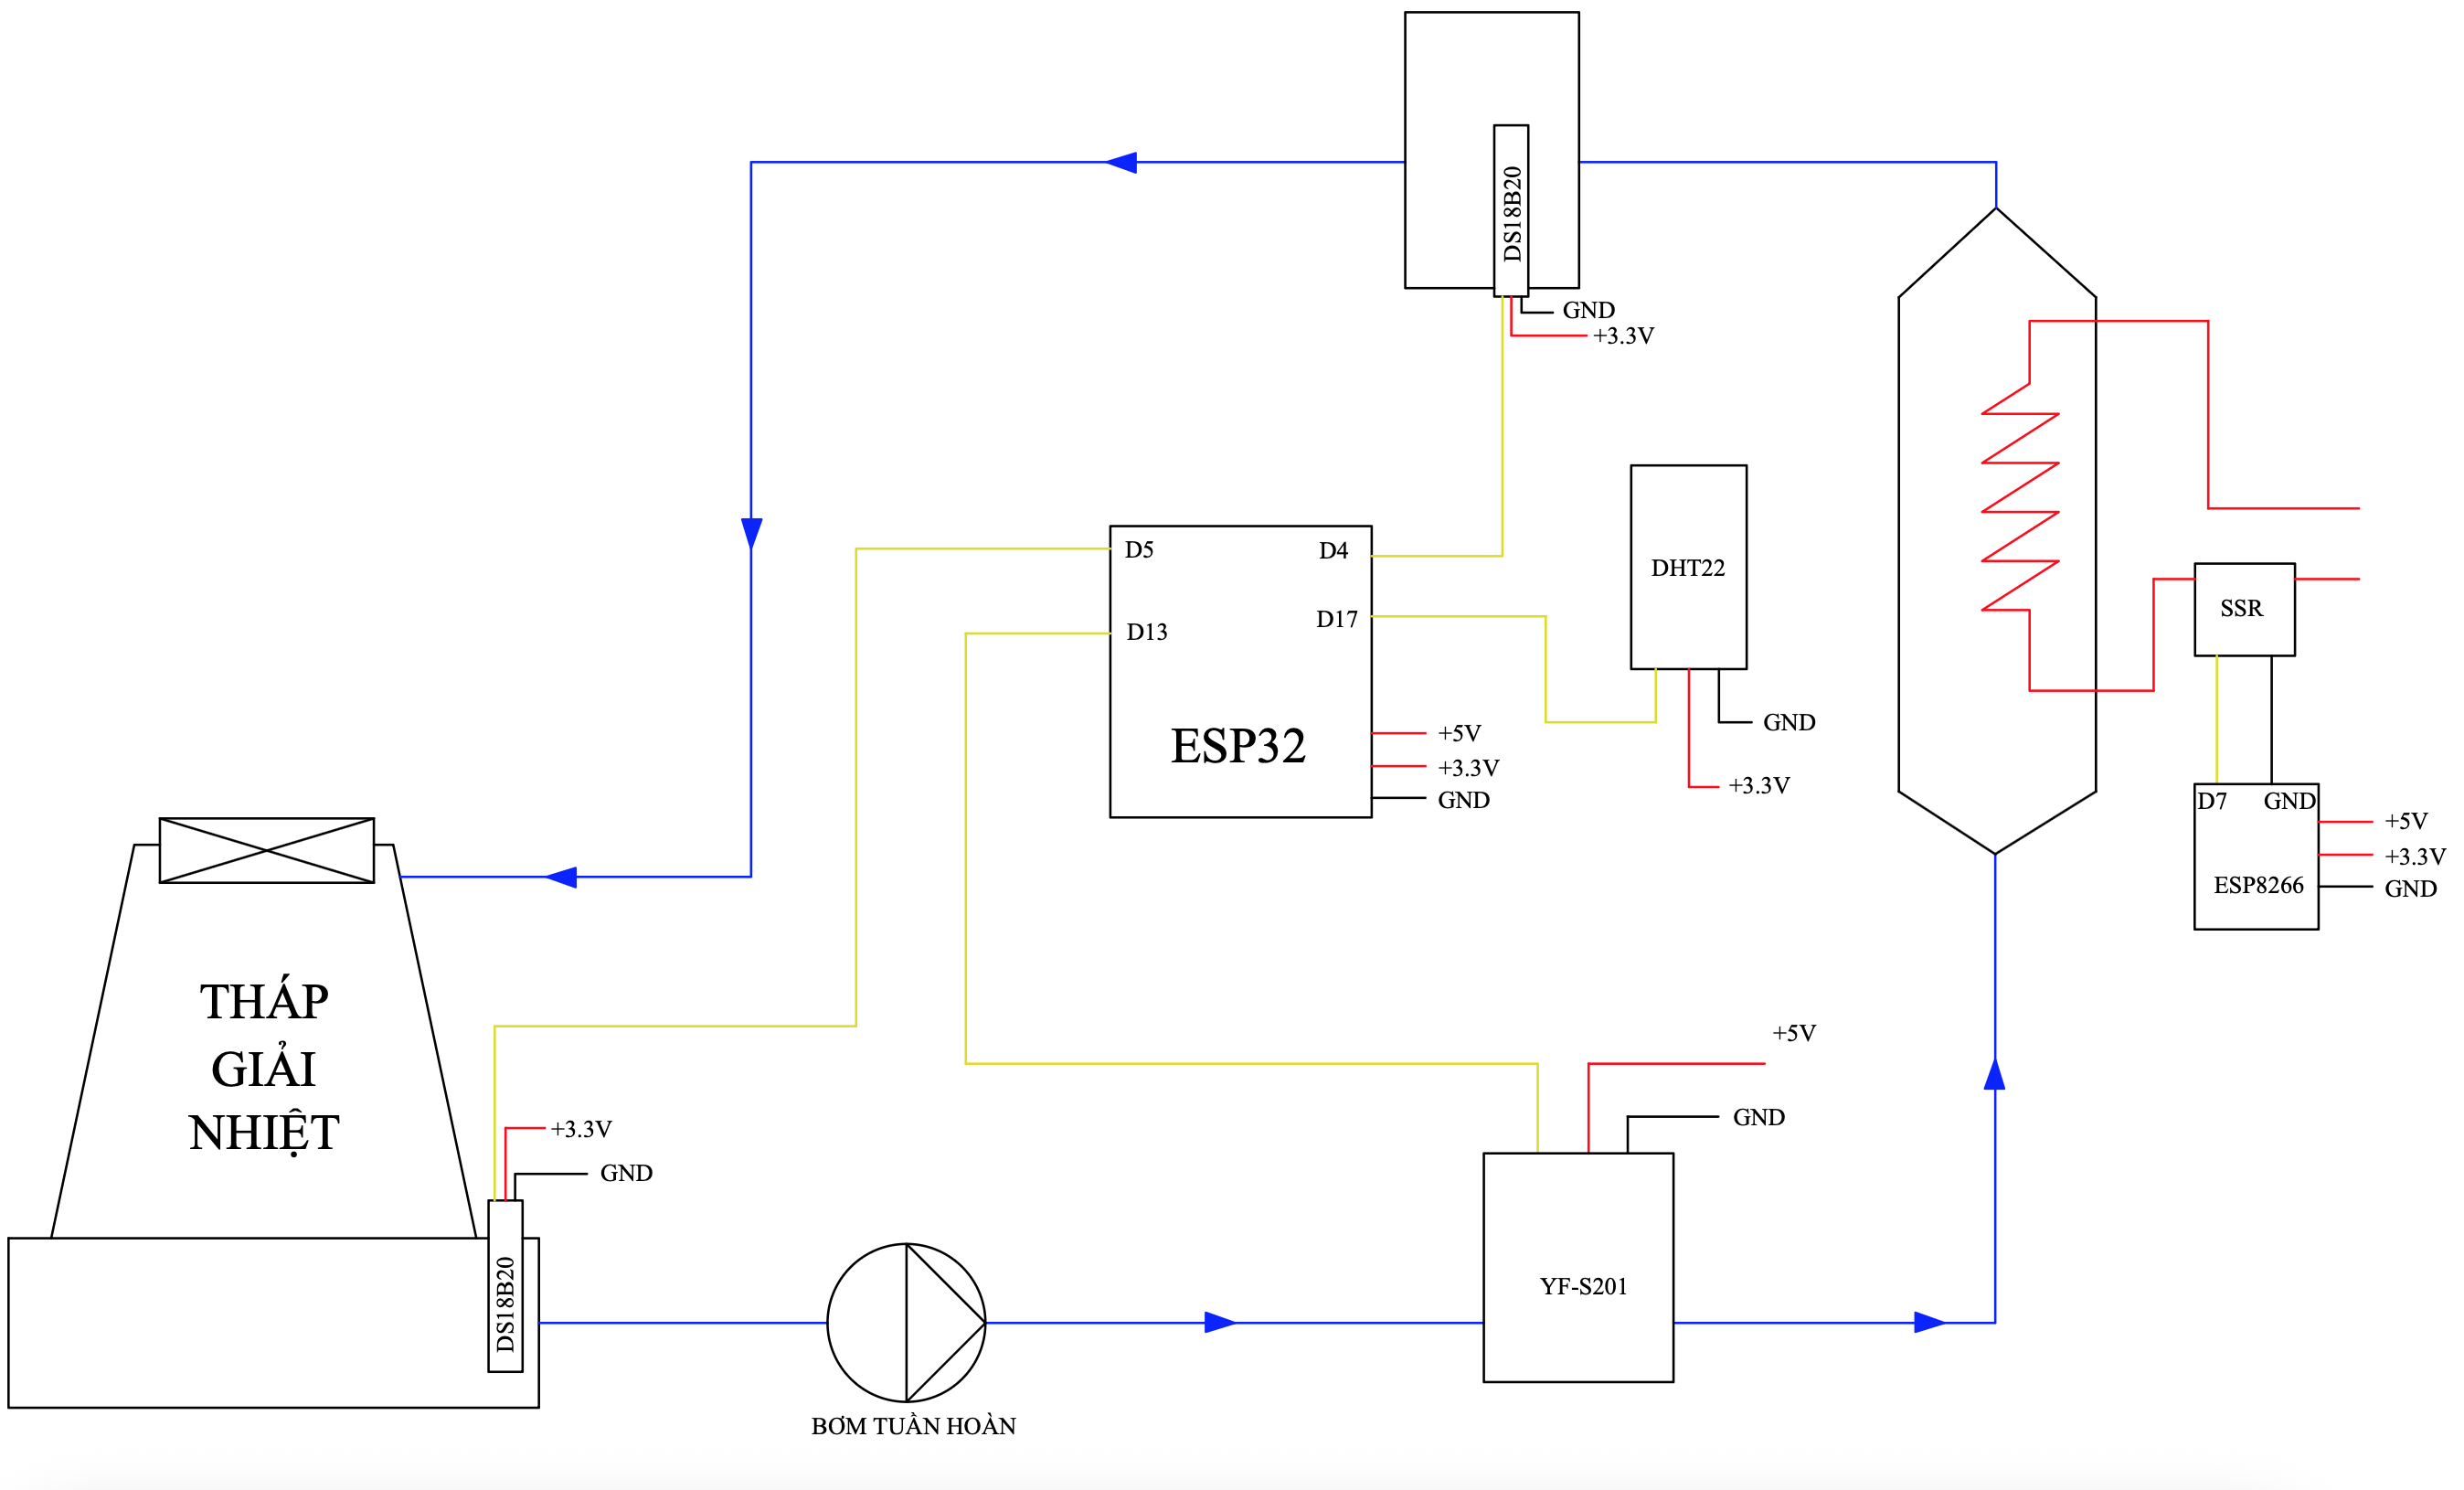
\includegraphics[width=1\textwidth]{Hinhve/so_do_dien.png}
    \caption{Sơ đồ cấu hình cảm biến và vi điều khiển vào mô hình thực tế}
    \label{fig:so_do_dien}
\end{figure}

Tổ hợp thiết bị ESP32, DS18B20, DHT22 và YF-S201 tạo giải pháp cân bằng tối ưu giữa yêu cầu kỹ thuật và tính khả thi kinh tế trong phạm vi mô hình thí nghiệm. Các hạn chế về độ chính xác được khắc phục qua hiệu chuẩn hiện trường, phương pháp trung bình hóa thống kê và lọc tín hiệu. Cấu trúc kết nối đơn giản góp phần rút ngắn thời gian triển khai và nâng cao độ tin cậy vận hành \cite{Espressif_ESP32_technical_reference,datasheet_DS18B20,datasheet_DHT22,datasheet_YFS201,ashrae2020cooling,epa_watersense_cooling_towers_2012}.

\section{Thiết kế kiến trúc phần mềm}
\label{sec:software_design}

Kiến trúc phần mềm của hệ thống giám sát tháp giải nhiệt được thiết kế theo mô hình phân tầng, trong đó dữ liệu được xử lý qua các giai đoạn tuần tự từ thu thập tại thiết bị biên đến trực quan hóa cuối cùng. Luồng xử lý chính bao gồm thu thập dữ liệu từ cảm biến bằng ESP32, truyền tải qua giao thức MQTT, xử lý trung tâm tại backend, lưu trữ trong InfluxDB và trực quan hóa thông qua Grafana.

\subsection{Phần mềm nhúng trên ESP32}
\label{sec:esp32_software}

Phần mềm nhúng trên ESP32 đóng vai trò đầu vào của toàn bộ hệ thống, chịu trách nhiệm thu thập dữ liệu từ các cảm biến và thực hiện xử lý sơ bộ trước khi truyền tải. Kiến trúc phần mềm được xây dựng trên nền tảng Arduino với thiết kế đa tác vụ tận dụng khả năng xử lý song song của vi điều khiển dual-core.

\begin{figure}
    \centering
    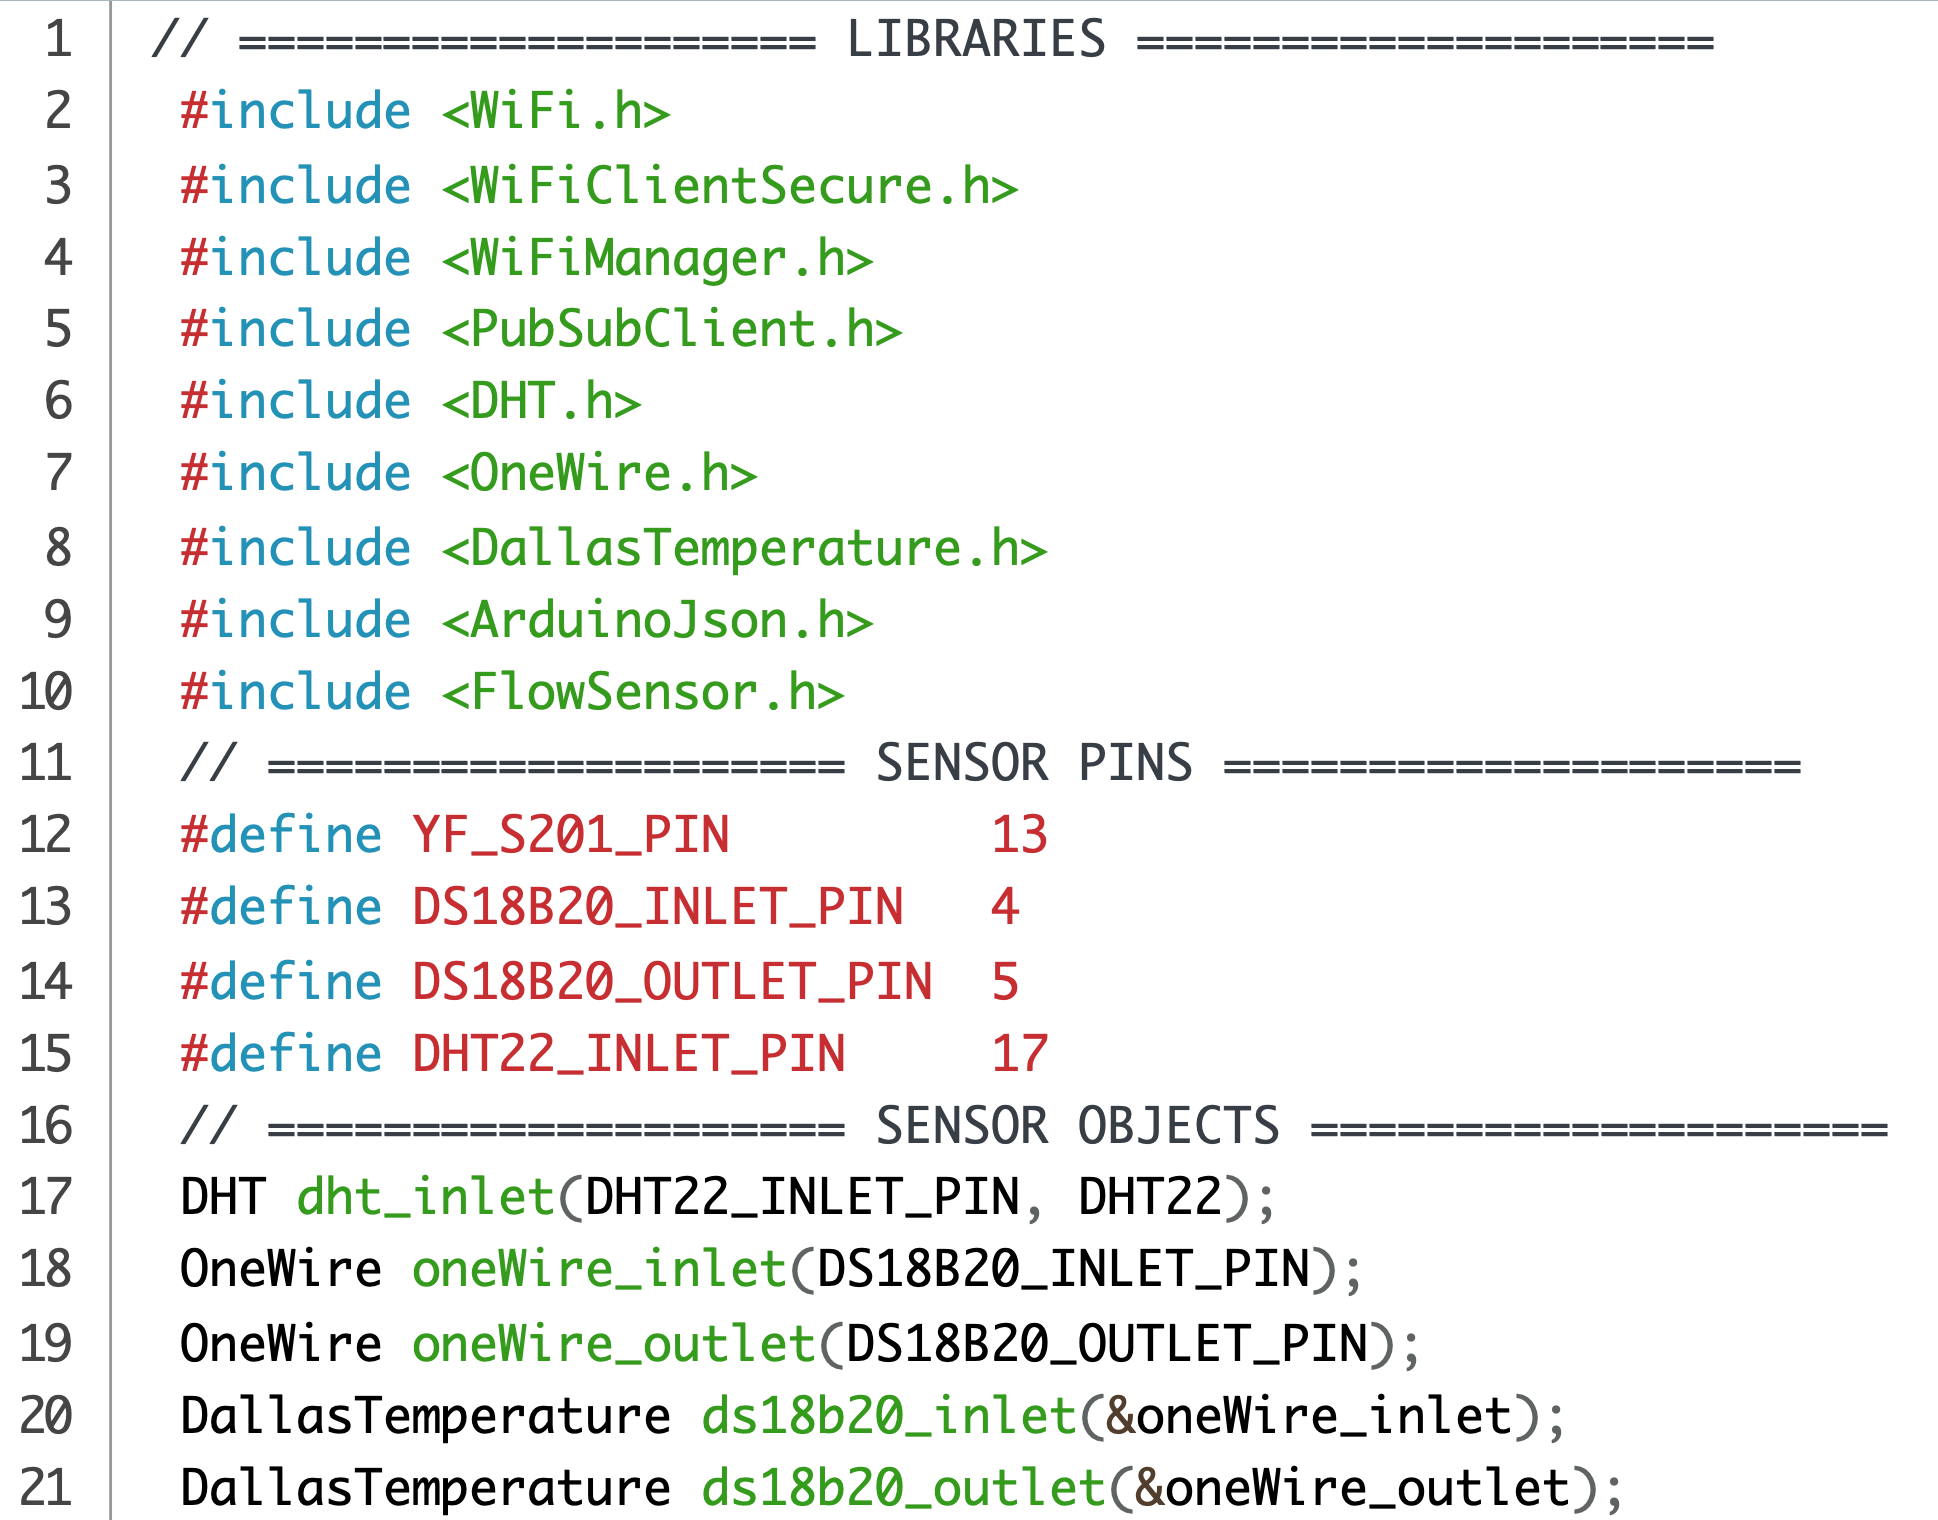
\includegraphics[width=0.8\textwidth]{../Hinhve/nhung_esp.png}
    \caption{Cấu trúc phần mềm nhúng ESP32 với khai báo thư viện và cấu hình hệ thống}
    \label{fig:esp32_firmware}
\end{figure}

Hệ thống phần mềm tích hợp các thư viện chuyên biệt bao gồm OneWire và DallasTemperature cho giao tiếp cảm biến nhiệt độ DS18B20, thư viện DHT22 cho đo lường độ ẩm và nhiệt độ không khí, WiFiManager quản lý kết nối mạng tự động, PubSubClient hỗ trợ giao thức MQTT bảo mật, ArduinoJson xử lý tuần tự hóa dữ liệu và WiFiClientSecure đảm bảo truyền thông mã hóa TLS.

Kiến trúc đa tác vụ phân chia xử lý trên hai lõi để tối ưu hiệu suất. Lõi chính đảm nhận thu thập dữ liệu cảm biến với chu kỳ định thời, xử lý và lọc nhiễu tín hiệu. Lõi phụ quản lý kết nối mạng, giao thức MQTT và các tác vụ truyền thông, đảm bảo việc thu thập dữ liệu không bị gián đoạn bởi hoạt động mạng.

Quy trình xử lý dữ liệu tại thiết bị bao gồm kiểm tra tính hợp lệ thông qua ngưỡng giá trị và mã kiểm tra, áp dụng bộ lọc số phù hợp với đặc tính từng loại cảm biến, thực hiện chuyển đổi đơn vị và hiệu chuẩn nhiệt độ. Dữ liệu được đóng gói định dạng JSON với dấu thời gian chính xác và thông tin trạng thái thiết bị trước khi truyền tải.

Cơ chế chống lỗi đa tầng bao gồm watchdog timer phần cứng, quy trình phục hồi tự động cho kết nối mạng và MQTT, cùng với hệ thống giám sát liên tục các thành phần chính. Thiết kế này đảm bảo hoạt động ổn định trong môi trường công nghiệp khắc nghiệt với khả năng tự khôi phục khi gặp sự cố.

\subsection{Giao thức truyền thông MQTT}
\label{sec:mqtt_protocol}

MQTT được lựa chọn làm giao thức truyền thông giữa ESP32 và hệ thống backend dựa trên ưu thế về hiệu suất băng thông thấp và độ tin cậy cao trong môi trường IoT. Giao thức hoạt động theo mô hình publish/subscribe, tạo sự tách biệt hoàn toàn giữa thiết bị gửi và nhận dữ liệu thông qua broker trung gian.

\begin{figure}[H]
    \centering
    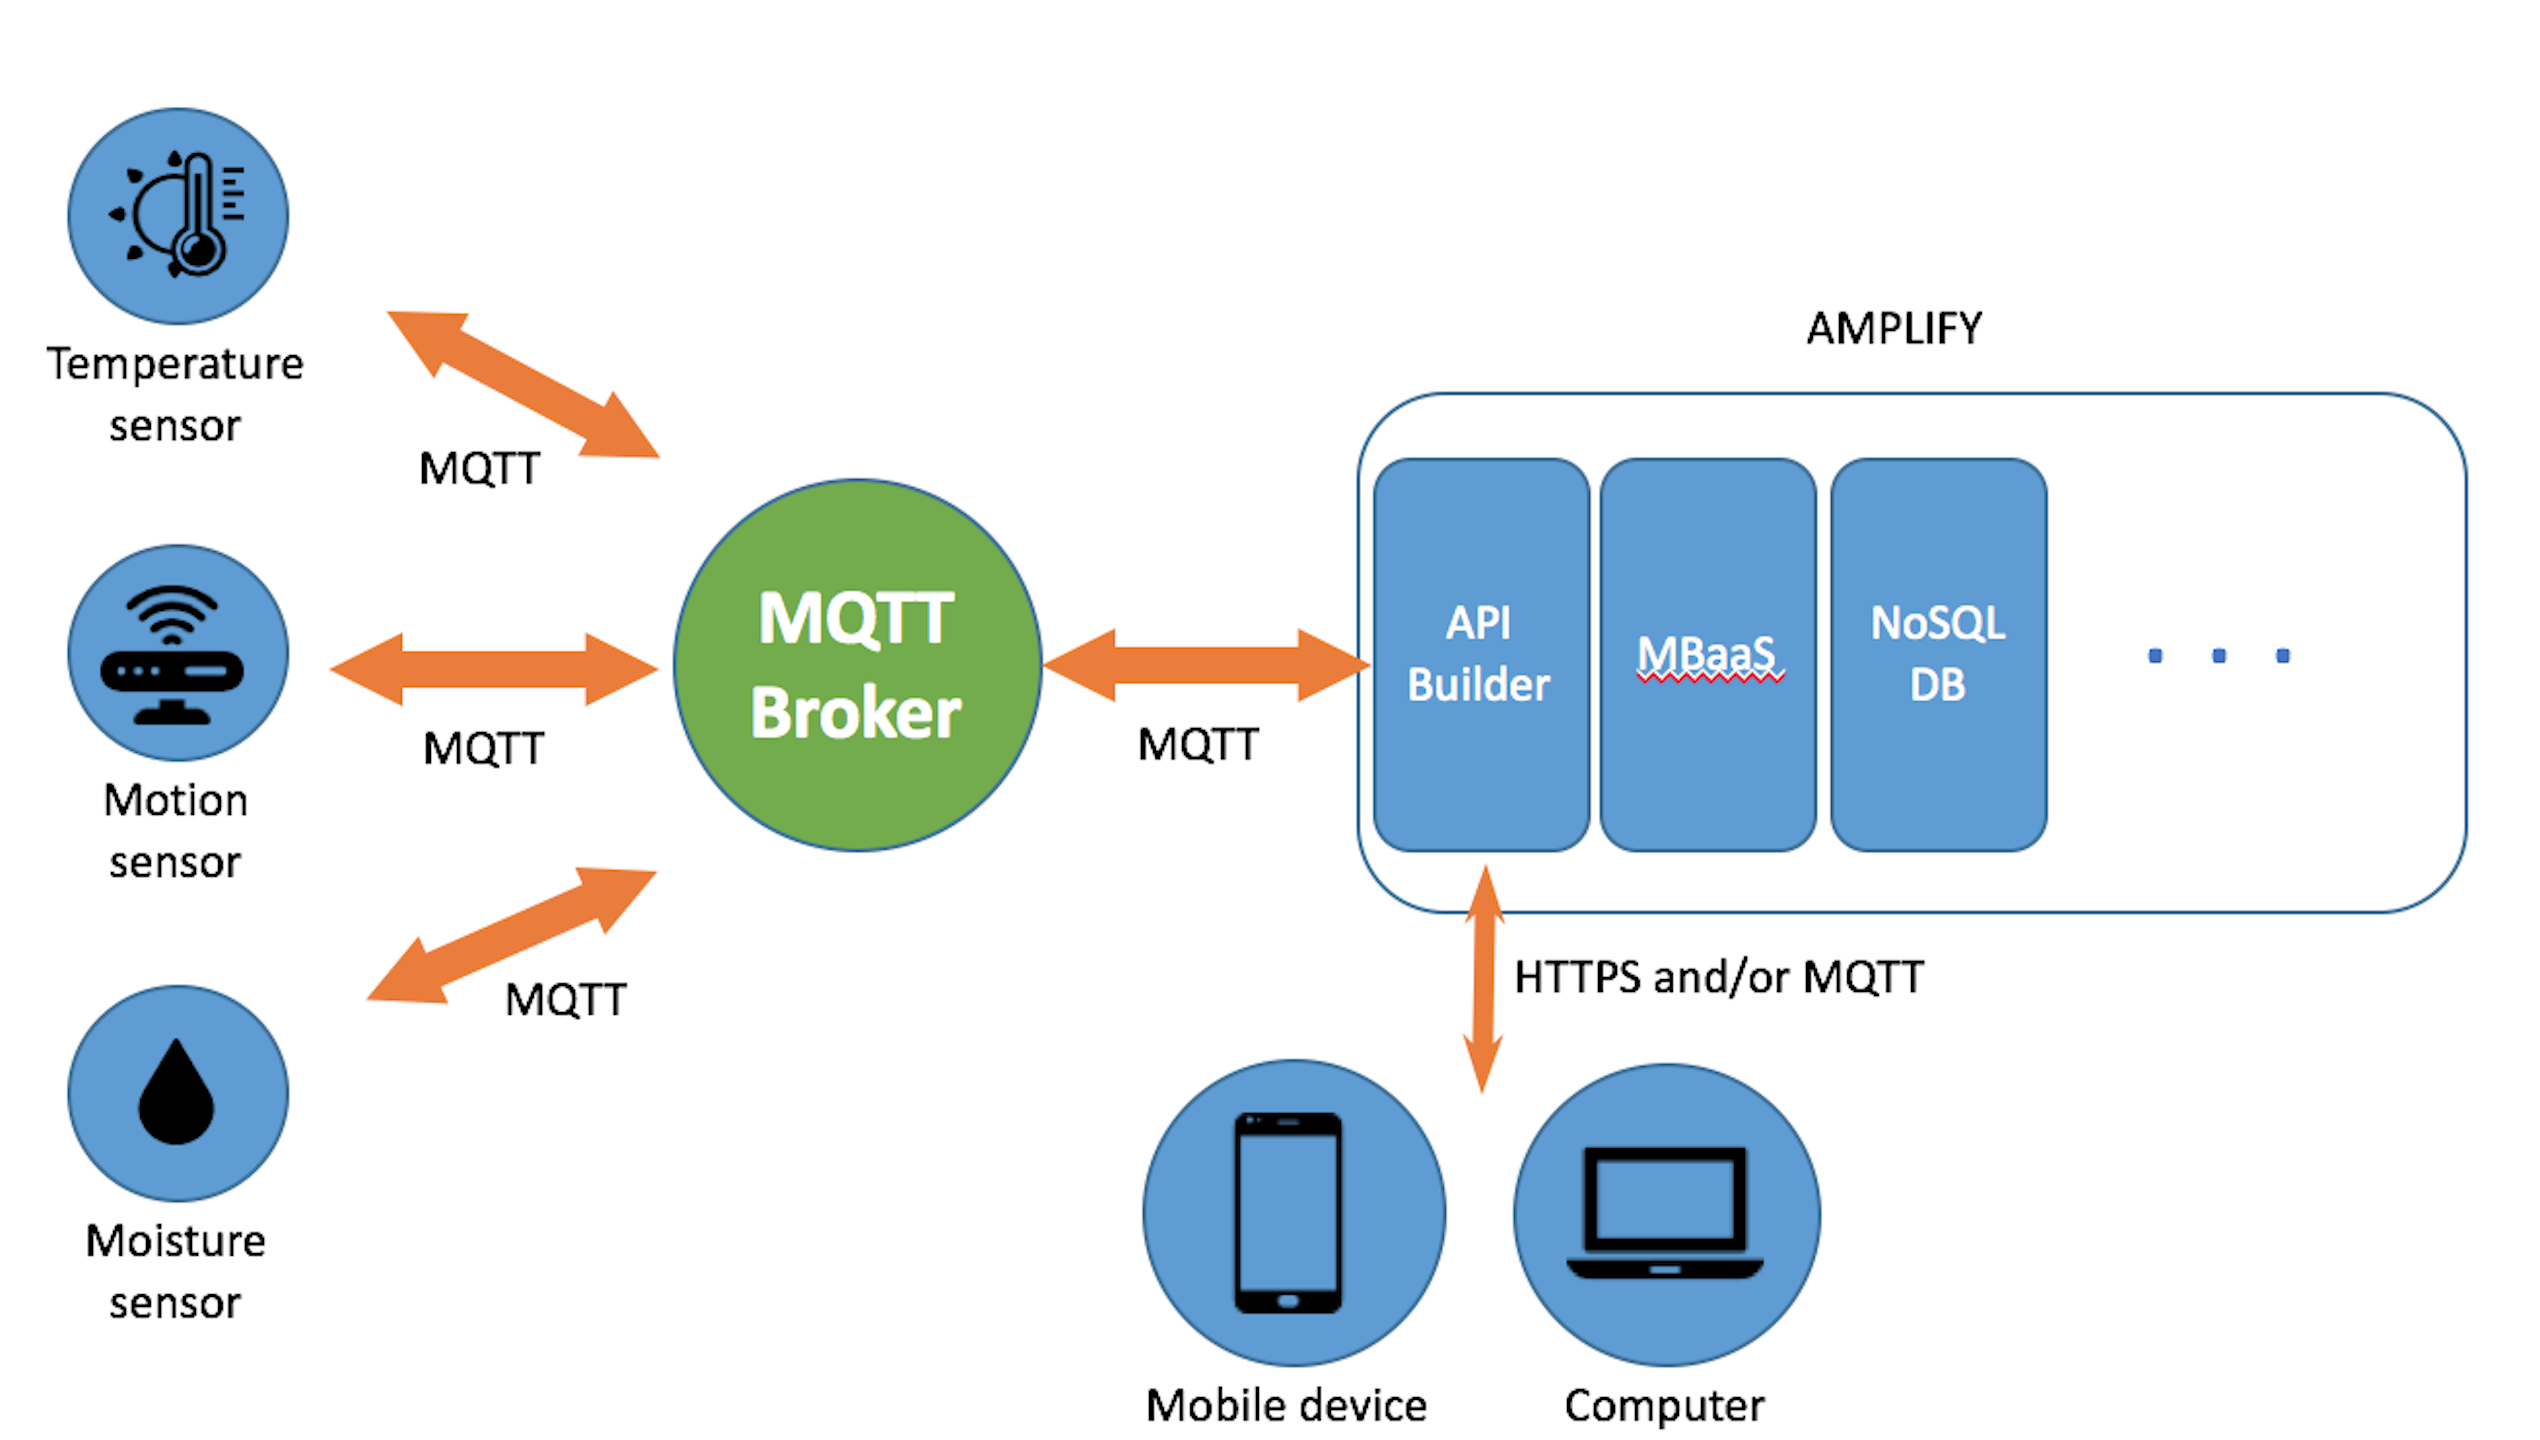
\includegraphics[width=1\textwidth]{../Hinhve/MQTT.png}
    \caption{Kiến trúc giao thức MQTT trong hệ thống giám sát}
    \label{fig:mqtt_model}
\end{figure}

Ưu thế chính của MQTT trong ứng dụng giám sát tháp giải nhiệt là khả năng truyền dữ liệu với overhead tối thiểu, phù hợp cho môi trường mạng có băng thông hạn chế. Giao thức cung cấp ba mức Quality of Service (QoS 0, 1, 2) đảm bảo độ tin cậy truyền dữ liệu từ cơ bản đến đảm bảo chính xác một lần, cho phép tối ưu theo yêu cầu cụ thể.

Tính năng session persistence đặc biệt quan trọng trong môi trường công nghiệp, duy trì trạng thái kết nối và buffer tạm thời các message khi thiết bị mất kết nối do sự cố mạng hoặc bảo trì. Cơ chế này đảm bảo không mất dữ liệu quan trọng và tự động đồng bộ khi kết nối được phục hồi.

Bảo mật được triển khai thông qua mã hóa TLS end-to-end và xác thực bằng username/password hoặc certificate. Cấu trúc topic được thiết kế đơn giản với \texttt{sensors/cooling\_tower} làm topic chính truyền tải toàn bộ dữ liệu cảm biến. Dữ liệu JSON bao gồm lưu lượng nước, nhiệt độ nước vào/ra, nhiệt độ và độ ẩm không khí, cùng metadata thiết bị và timestamp.

\subsection{Hệ thống backend xử lý dữ liệu}
\label{sec:backend_system}

Hệ thống backend đóng vai trò trung tâm xử lý dữ liệu, hoạt động như cầu nối thông minh giữa MQTT broker và cơ sở dữ liệu InfluxDB. Được phát triển bằng Python, hệ thống đảm nhận các chức năng tính toán phức tạp vượt quá khả năng xử lý của vi điều khiển ESP32.

\begin{figure} [H]
    \centering
    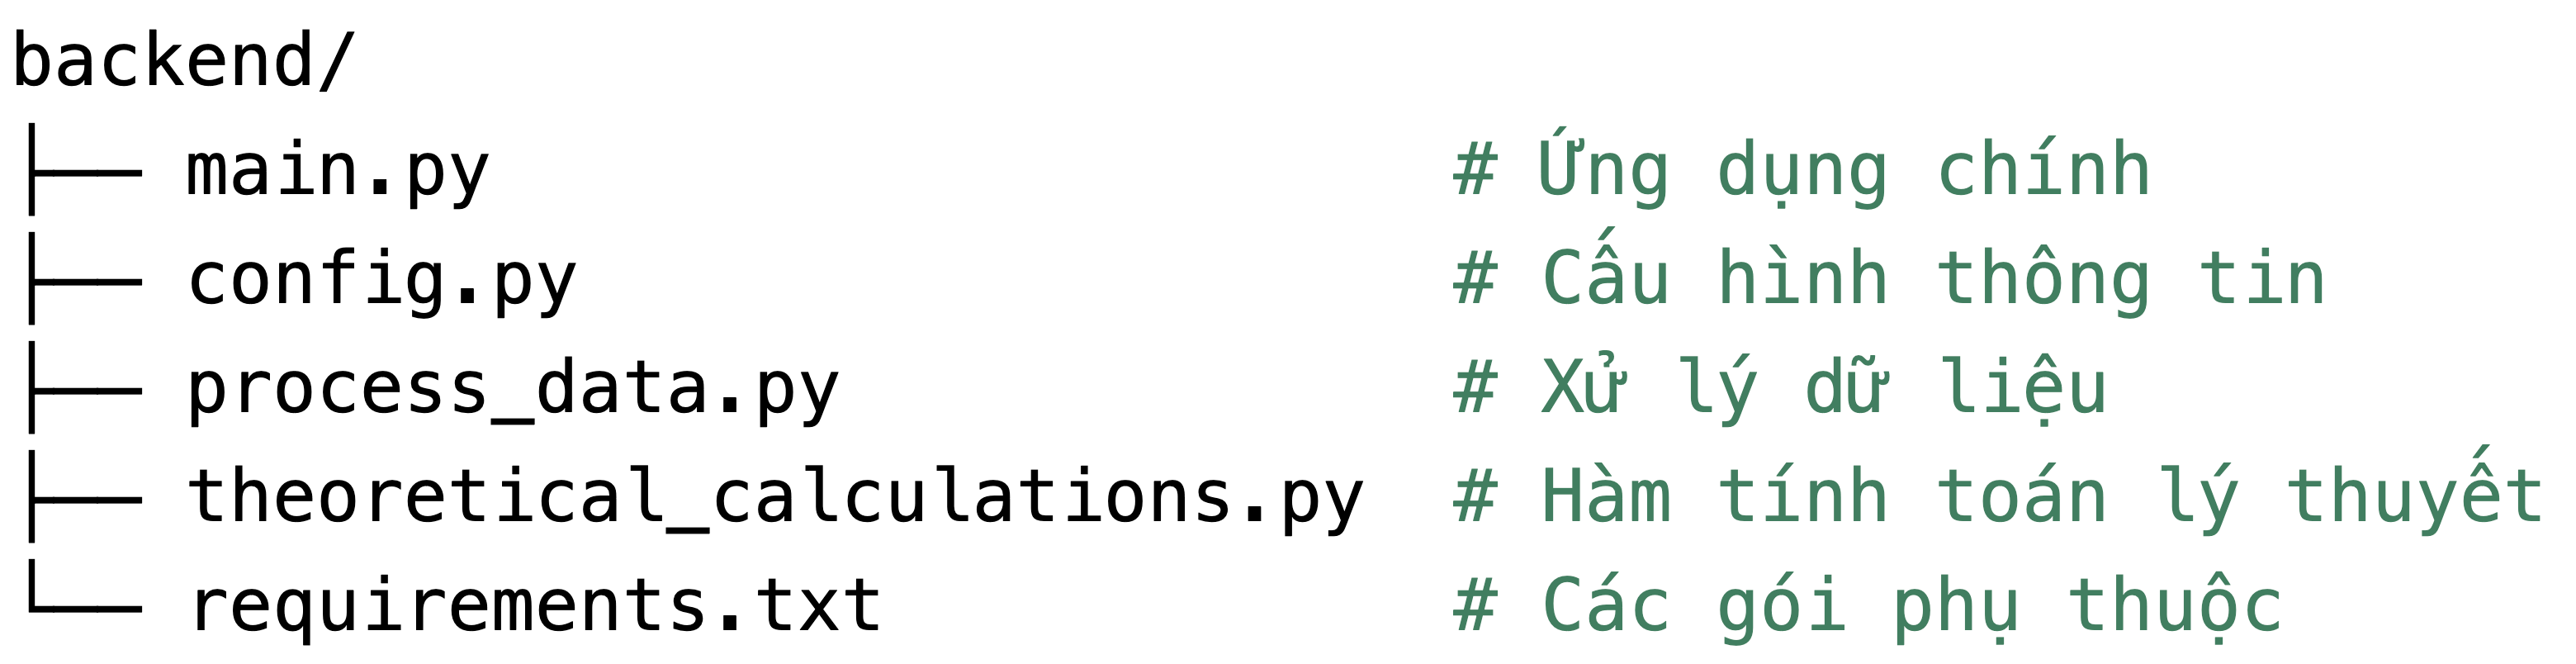
\includegraphics[width=0.8\textwidth]{../Hinhve/backend.png}
    \caption{Kiến trúc hệ thống backend với các thành phần xử lý}
    \label{fig:backend_architecture}
\end{figure}

Kiến trúc modular với phân tách rõ ràng các thành phần chức năng: MQTT subscriber nhận dữ liệu từ broker, data processor thực hiện lọc nhiễu và validation, calculation engine áp dụng các công thức lý thuyết phức tạp, database interface quản lý giao tiếp InfluxDB, monitoring module phát hiện bất thường và alerting system gửi cảnh báo kịp thời.

Chức năng cốt lõi bao gồm tiếp nhận dữ liệu real-time từ MQTT topic, validation và preprocessing đảm bảo chất lượng dữ liệu, áp dụng công thức Stull tính toán nhiệt độ bầu ướt và các thông số hiệu suất tháp giải nhiệt, lưu trữ dữ liệu thô và processed vào InfluxDB với schema tối ưu, phân tích xu hướng hỗ trợ predictive maintenance và cung cấp API endpoints cho giao diện người dùng.

Hệ thống tích hợp cơ chế error handling toàn diện với retry logic cho kết nối database, circuit breaker pattern cho external services, comprehensive logging và health monitoring. Thiết kế này đảm bảo độ tin cậy cao và khả năng phục hồi tự động trong môi trường production.

\subsection{Cơ sở dữ liệu InfluxDB}
\label{sec:influxdb_database}

InfluxDB được triển khai làm hệ thống lưu trữ chuyên biệt cho dữ liệu time-series, tối ưu hóa cho việc ghi dữ liệu tần suất cao và truy vấn hiệu quả. Kiến trúc columnar cho phép xử lý hàng triệu data points mỗi giây với khả năng nén dữ liệu 90-95\% so với dung lượng gốc.

\begin{figure}
    \centering
    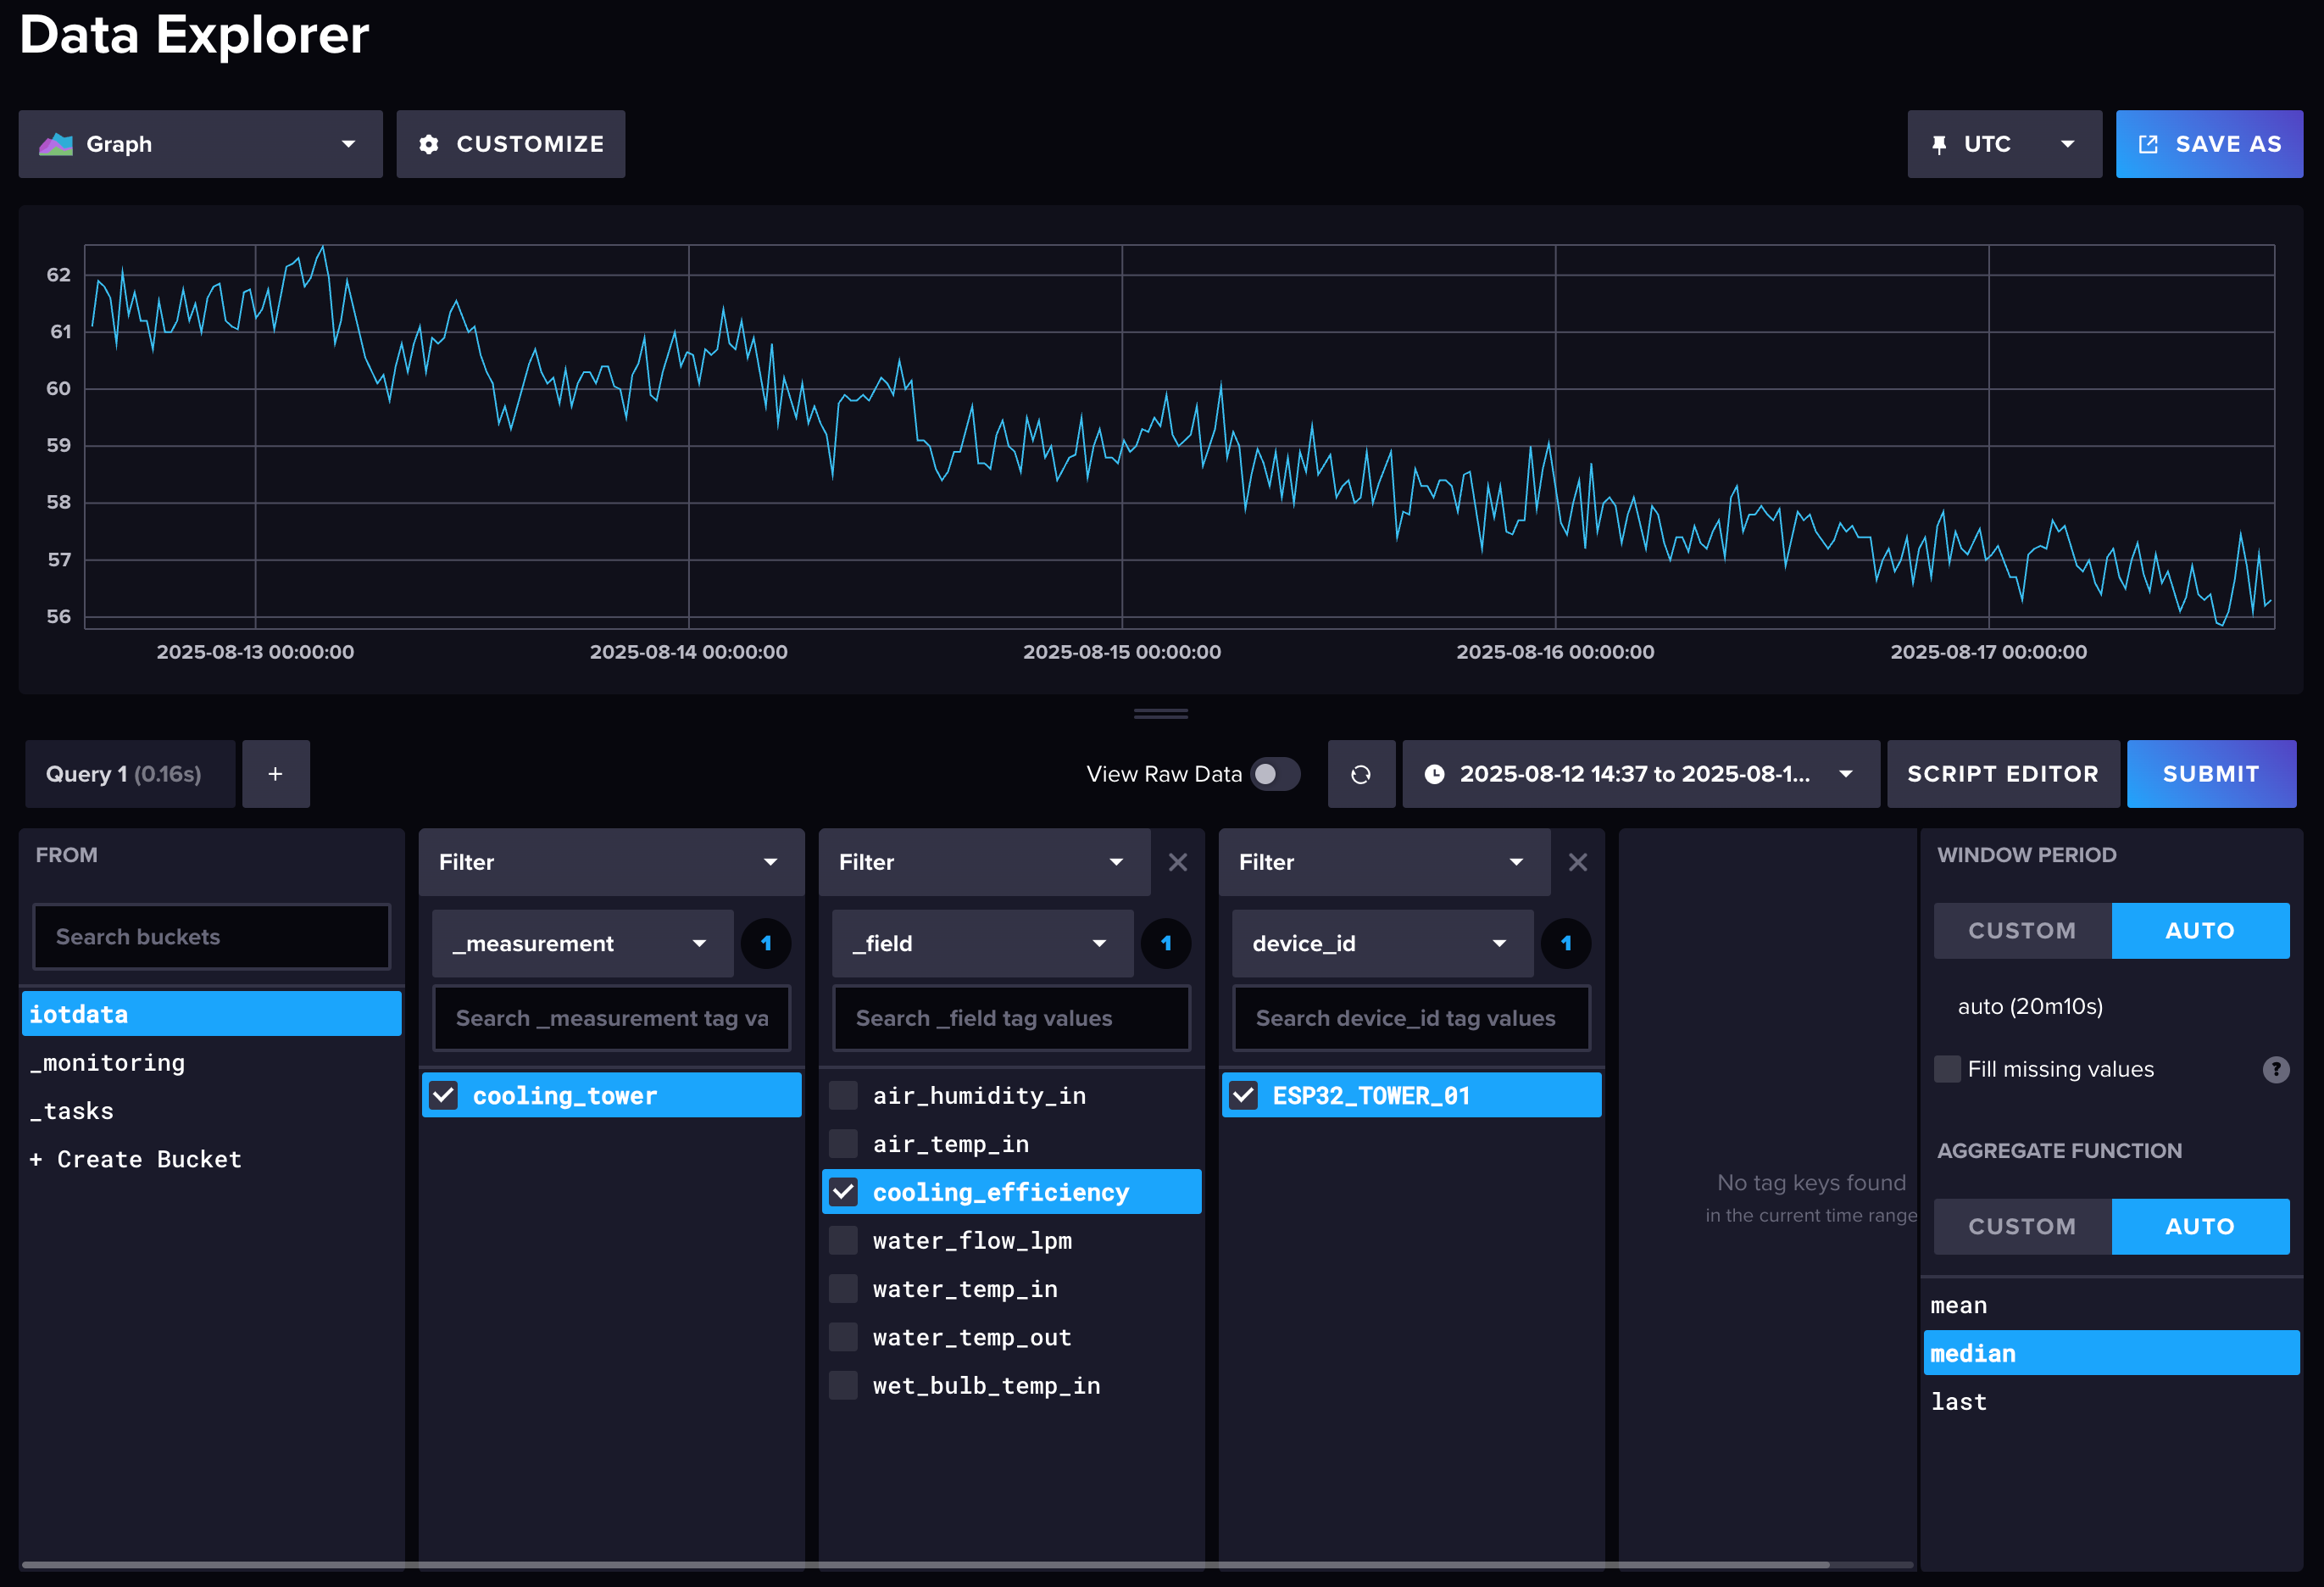
\includegraphics[width=1\textwidth]{../Hinhve/influxdb.png}
    \caption{Kiến trúc lưu trữ dữ liệu time-series với InfluxDB}
    \label{fig:influxdb_architecture}
\end{figure}

Cấu trúc dữ liệu được tổ chức theo measurements làm đơn vị chính cho dữ liệu cảm biến, tags để indexing và grouping theo tiêu chí như sensor type và location, fields chứa giá trị thực tế của phép đo và timestamps với độ chính xác nanosecond. Schema được thiết kế để tối ưu cho các truy vấn phân tích xu hướng và aggregation theo thời gian.

Retention policies quản lý lifecycle dữ liệu tự động, xóa dữ liệu cũ theo quy tắc định nghĩa trước để tối ưu storage. Continuous queries thực hiện downsampling và pre-aggregation tự động, tính toán các thống kê như mean, max, min theo khoảng thời gian khác nhau mà không cần can thiệp thủ công.

Ngôn ngữ truy vấn InfluxQL với syntax tương tự SQL giúp giảm learning curve và tận dụng kiến thức sẵn có. Hệ thống hỗ trợ các chức năng nâng cao như mathematical functions, statistical analysis và time-based grouping phục vụ phân tích hiệu suất tháp giải nhiệt.

\subsection{Trực quan hóa dữ liệu với Grafana}
\label{sec:grafana_visualization}

Grafana đóng vai trò frontend cuối cùng trong chuỗi xử lý dữ liệu, cung cấp dashboard tương tác để trực quan hóa thông tin vận hành. Kết nối trực tiếp với InfluxDB cho phép hiển thị dữ liệu real-time và historical analysis với độ trễ tối thiểu.

\begin{figure}
    \centering
    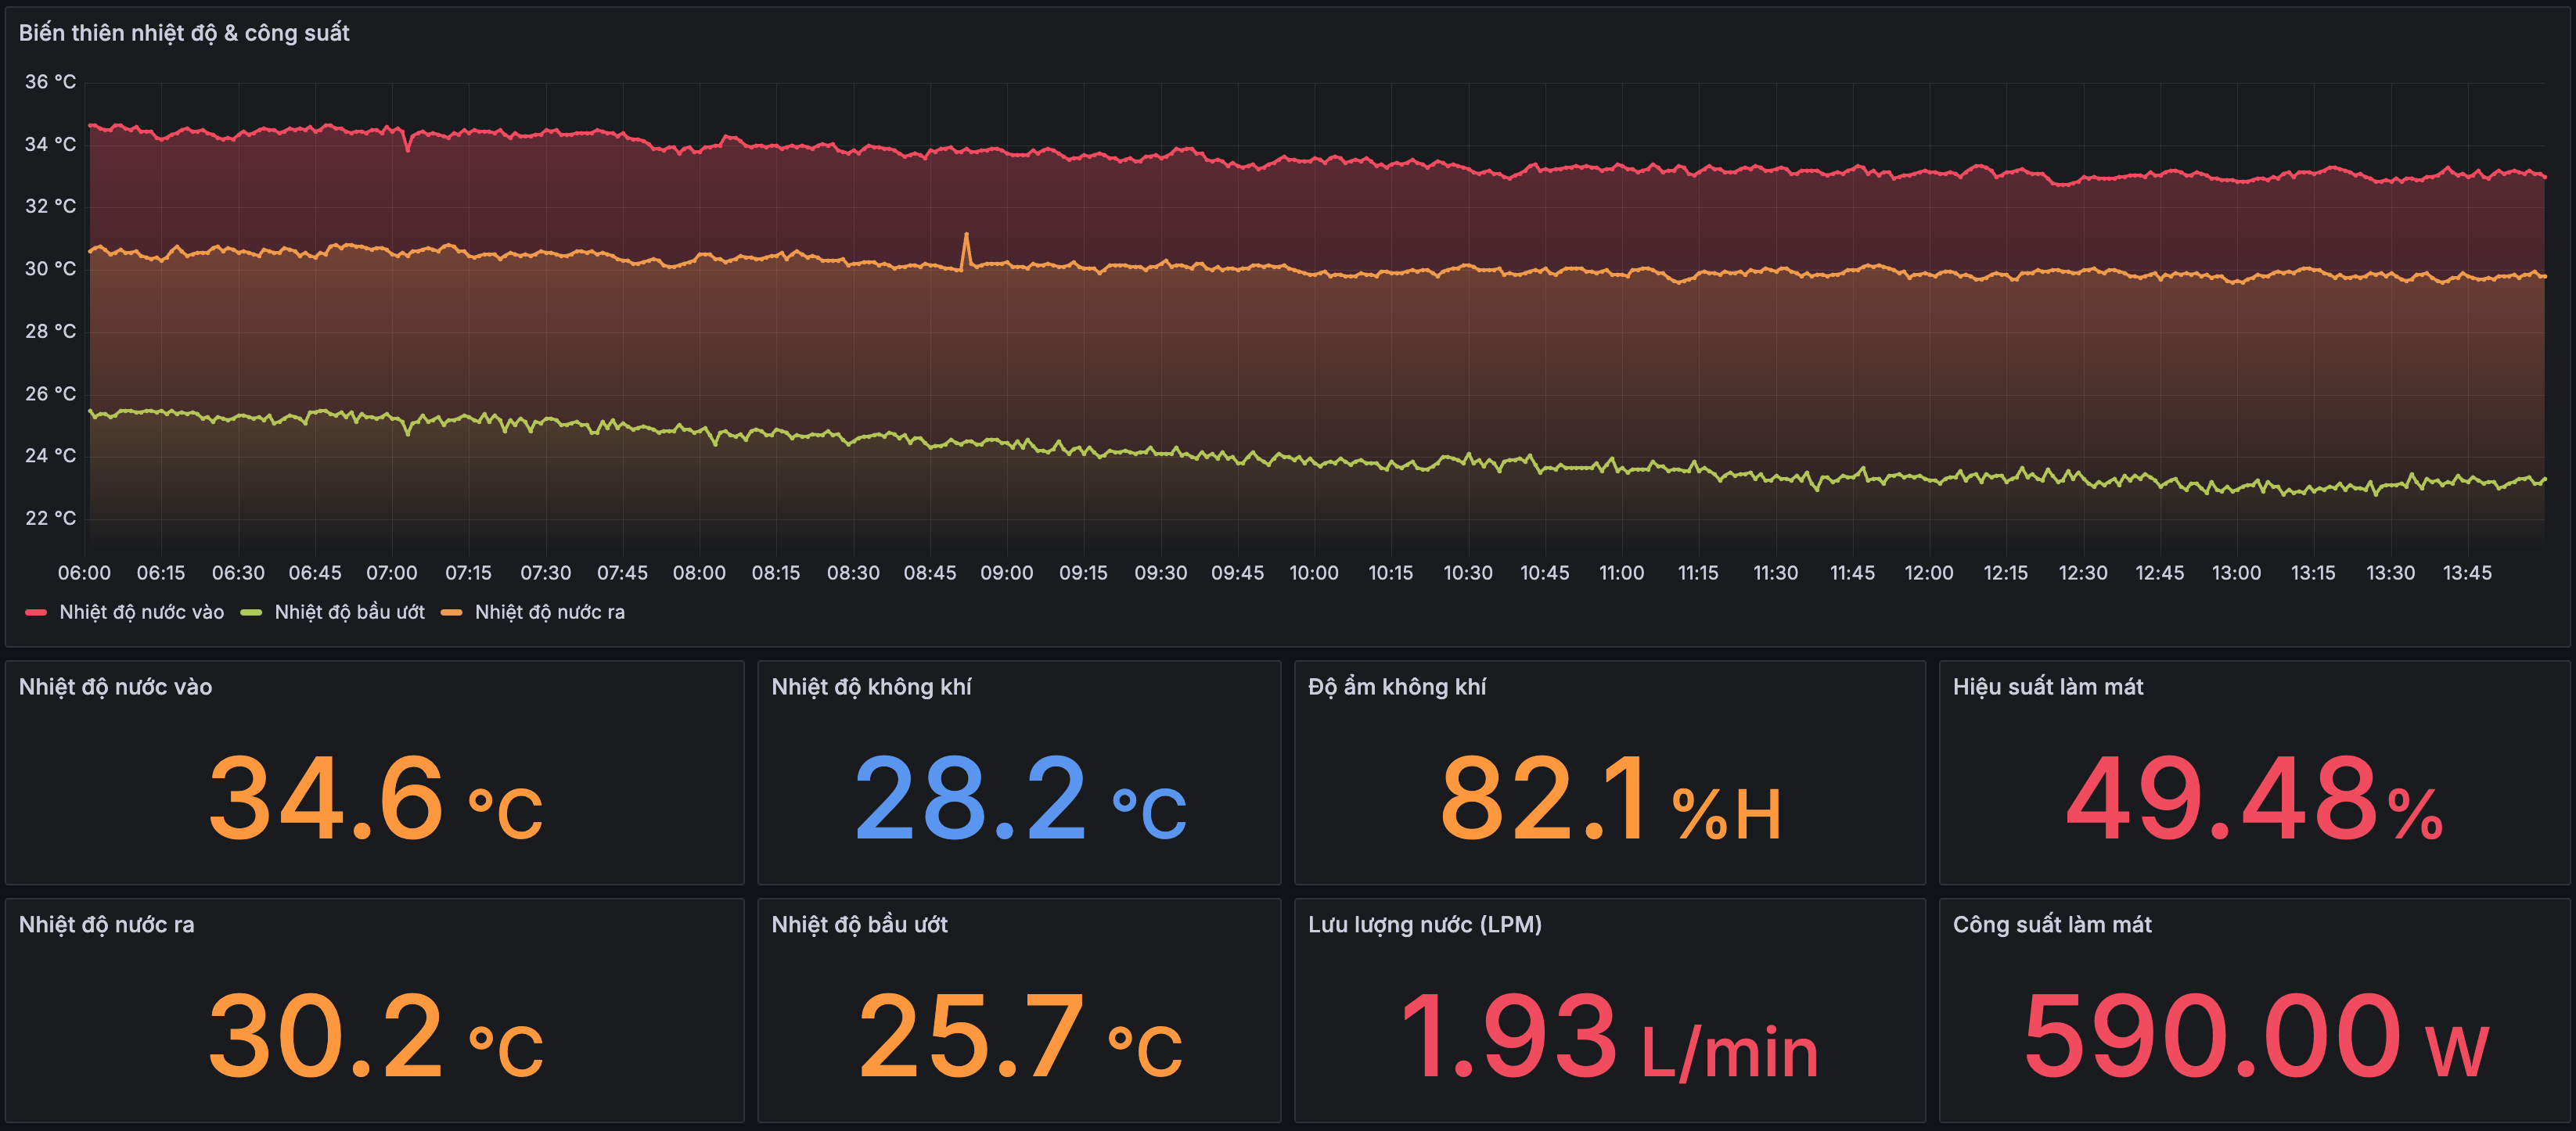
\includegraphics[width=1\textwidth]{../Hinhve/grafana_cap.png}
    \caption{Dashboard Grafana hiển thị dữ liệu giám sát tháp giải nhiệt}
    \label{fig:grafana_dashboard}
\end{figure}

Bảng điều khiển Grafana được xây dựng với cấu trúc các panel chức năng được tổ chức hợp lý, đảm bảo khả năng trực quan hóa và phân tích toàn diện dữ liệu vận hành của tháp giải nhiệt. Các biểu đồ chuỗi thời gian thể hiện rõ ràng sự biến thiên của công suất giải nhiệt, nhiệt độ nước vào, nước ra và nhiệt độ bầu ướt, từ đó hỗ trợ đánh giá liên tục hiệu suất làm mát của hệ thống. Các panel số liệu cung cấp thông tin tức thời về các chỉ số vận hành trọng yếu, giúp người vận hành nhận diện nhanh trạng thái hệ thống. Phần trực quan hóa lưu lượng nước cho phép đánh giá chính xác tình trạng hoạt động của hệ thống tuần hoàn. Bên cạnh đó, bảng thống kê tổng hợp dữ liệu theo từng khoảng thời gian được tích hợp nhằm phục vụ phân tích xu hướng và hỗ trợ công tác bảo trì dự báo. Các panel cảnh báo được thiết kế để phát hiện sớm các bất thường trong quá trình vận hành, góp phần nâng cao mức độ an toàn và độ tin cậy của hệ thống. Ngoài ra, chức năng phân tích tương quan giữa dữ liệu vận hành và điều kiện thời tiết cũng được triển khai, tạo điều kiện thuận lợi cho việc đánh giá và tối ưu hóa hiệu suất tổng thể của tháp giải nhiệt.

Hệ thống dashboard hỗ trợ giám sát thời gian thực với cơ chế tự động làm mới dữ liệu, đồng thời cho phép truy xuất và phân tích dữ liệu lịch sử. Giao diện được thiết kế thích ứng với nhiều loại thiết bị, bao gồm cả máy tính và thiết bị di động, đồng thời hỗ trợ xuất dữ liệu dưới nhiều định dạng khác nhau phục vụ nhu cầu báo cáo ngoại tuyến. Trải nghiệm người dùng được chú trọng tối ưu hóa, đảm bảo các thông tin quan trọng được trình bày trực quan, hỗ trợ hiệu quả cho quá trình ra quyết định vận hành và bảo trì hệ thống.

\section{Triển khai và tích hợp hệ thống}
\label{sec:system_implementation}

\subsection{Luồng hoạt động tổng thể}
\label{sec:system_workflow}

Hệ thống giám sát hoạt động theo một quy trình làm việc được tối ưu hóa để đảm bảo tính liên tục và độ tin cậy của dữ liệu. Quy trình bắt đầu từ việc ESP32 thực hiện thu thập dữ liệu từ tất cả cảm biến với chu kỳ được tối ưu, tiếp theo là xử lý sơ bộ bao gồm kiểm tra tính hợp lệ, lọc nhiễu và đóng gói dữ liệu theo định dạng JSON trước khi truyền lên bộ điều phối MQTT qua kết nối mạng không dây Wi-Fi được bảo mật.

\begin{figure}[H]
    \centering
    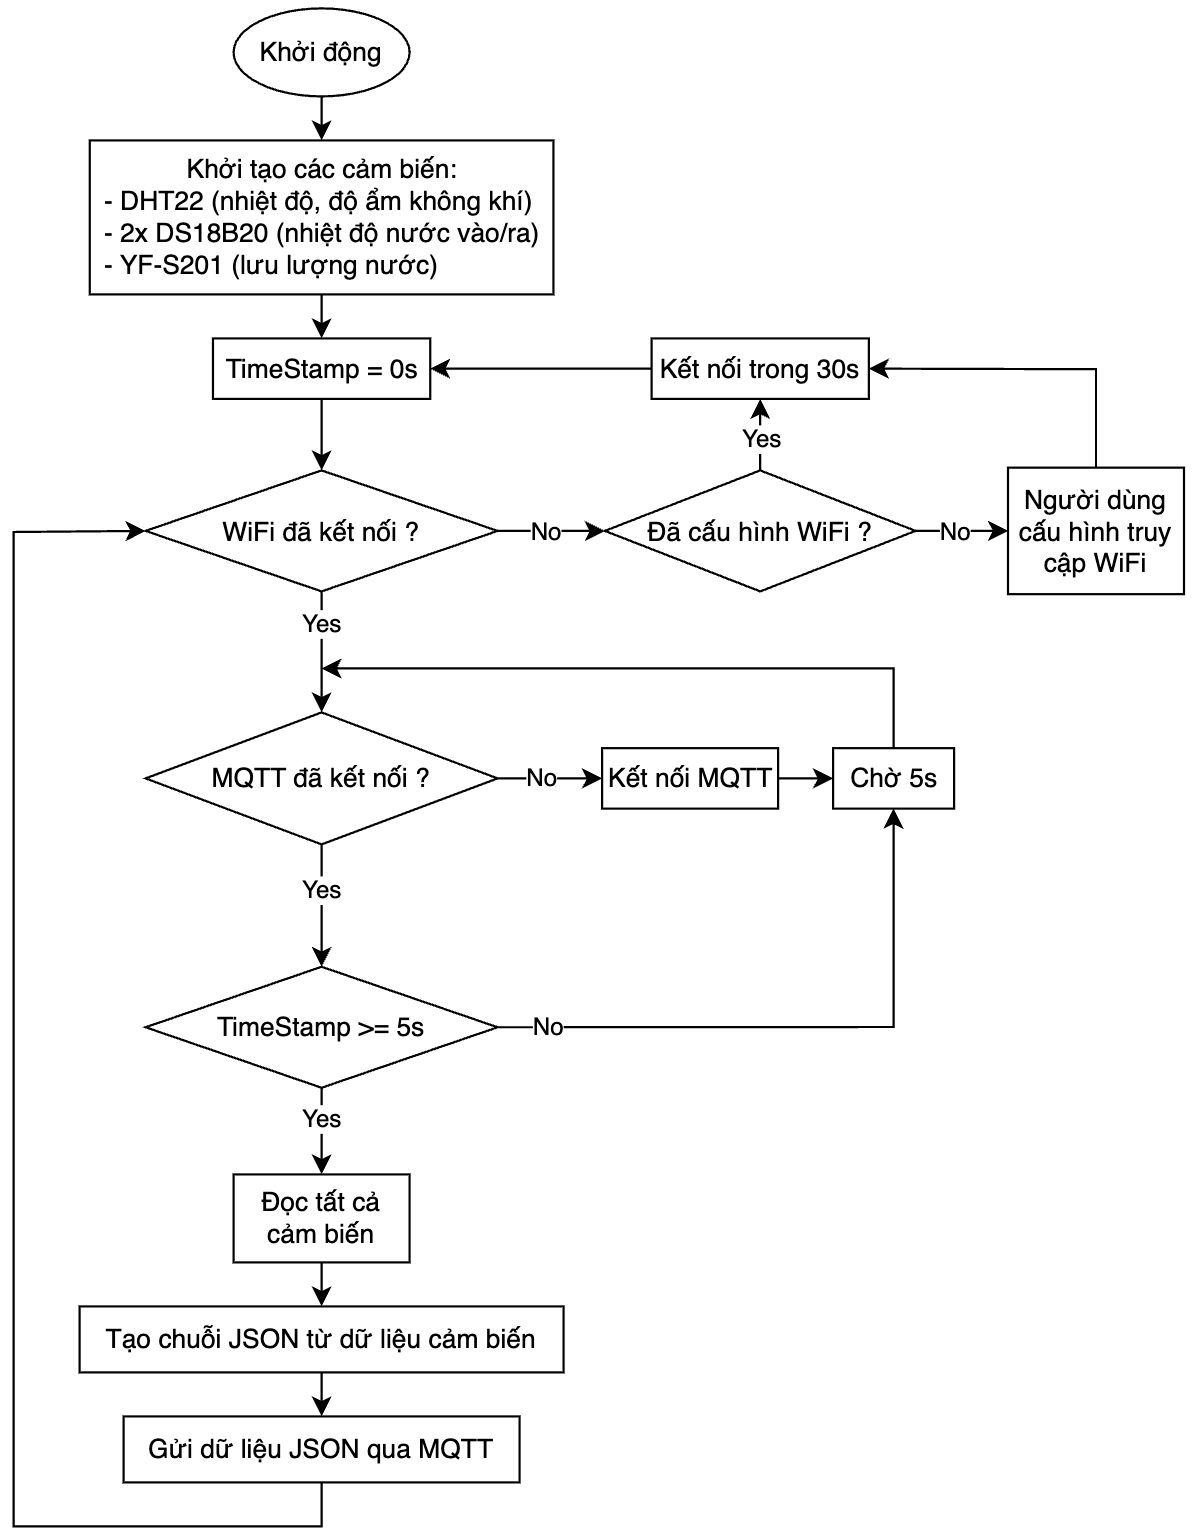
\includegraphics[width=1\textwidth]{../Hinhve/esp_block.png}
    \caption{Lưu đồ thuật toán xử lý dữ liệu và truyền thông của ESP32 trong hệ thống giám sát tháp giải nhiệt}
    \label{fig:system_block_diagram}
\end{figure}

Hệ thống xử lý trung tâm đóng vai trò then chốt trong việc nhận và xử lý dữ liệu từ các chủ đề MQTT, thực hiện các tính toán phức tạp bao gồm nhiệt độ bầu ướt theo công thức Stull, công suất làm mát và hiệu suất tháp giải nhiệt theo các phương trình đã được trình bày trong chương 2. Dữ liệu sau khi được xử lý sẽ được lưu trữ vào InfluxDB với cấu trúc được tối ưu cho dữ liệu chuỗi thời gian.

Bảng điều khiển Grafana cung cấp giao diện trực quan cho người vận hành với khả năng hiển thị giám sát thời gian thực, phân tích xu hướng lịch sử và cảnh báo thông minh. Hệ thống được trang bị các cơ chế chống lỗi bao gồm tự động kết nối lại khi mất mạng, lưu trữ dữ liệu tạm thời khi mất kết nối, giám sát tình trạng hoạt động và tự động phục hồi dịch vụ, cùng với các quy trình sao lưu và khôi phục sau sự cố.

\subsection{Thiết kế tích hợp phần cứng}
\label{sec:hardware_integration}

Phần này trình bày kiến trúc tích hợp phần cứng cho hệ thống giám sát tháp giải nhiệt, với trọng tâm là đảm bảo an toàn điện, tương thích điện từ (EMC)\footnote{Electromagnetic Compatibility (EMC) là khả năng của thiết bị điện tử hoạt động bình thường trong môi trường điện từ mà không gây nhiễu cho các thiết bị khác và không bị ảnh hưởng bởi nhiễu từ môi trường xung quanh, được quy định trong các tiêu chuẩn như IEC 61326 cho thiết bị đo lường điện.}, khả năng bảo trì và tối ưu hóa chi phí trong phạm vi \textit{mô hình thí nghiệm}\footnote{Các lựa chọn phần cứng trong mô hình thí nghiệm (ví dụ: bo mạch phát triển ESP32 có nguồn tích hợp, cảm biến cấp prototype) được tối ưu hóa cho tính đơn giản và chi phí thấp. Trong triển khai công nghiệp thực tế, cần sử dụng nguồn chuẩn công nghiệp (DIN-rail PSU tuân thủ IEC 61131-2), các biện pháp bảo vệ quá áp/sét lan truyền (IEC 61643), tiêu chuẩn bảo vệ IP65/IP67 (IEC 60529) và IK cao hơn, cách ly galvanic cho tín hiệu, cùng tuân thủ nghiêm ngặt các tiêu chuẩn an toàn điện (IEC 61010) và EMC (EN 61326) có liên quan.}. 

Kiến trúc tổng thể được xây dựng với ESP32 làm đơn vị xử lý trung tâm (chi tiết tại phần \textbf{\ref{sec:esp32_controller}}), kết nối với mạng lưới cảm biến đa tham số bao gồm: cảm biến nhiệt độ nước DS18B20 (phần \textbf{\ref{sec:ds18b20_sensor}}) tại các điểm đo chiến lược, cảm biến nhiệt độ--độ ẩm không khí DHT22 (phần \textbf{\ref{sec:dht22_sensor}}) để đánh giá điều kiện môi trường, và cảm biến lưu lượng nước tuần hoàn YF-S201 (phần \textbf{\ref{sec:yf_s201_sensor}}) cho việc tính toán cân bằng năng lượng. Hệ thống được thiết kế để vận hành ổn định trong các điều kiện môi trường khắc nghiệt đặc trưng của tháp giải nhiệt, bao gồm độ ẩm cao (RH > 80\%), sương nước ngưng tụ, và sự hiện diện của các hóa chất xử lý nước như clo và chất ức chế ăn mòn \cite{Espressif_ESP32_technical_reference,epa_watersense_cooling_towers_2012,ashrae2020cooling}.

\subsubsection{Tiêu chí và ràng buộc thiết kế}
Thiết kế kiến trúc phần cứng được định hướng theo các tiêu chí chính: (i) đảm bảo biên độ an toàn điện và tương thích điện từ (EMC) theo khuyến nghị của nhà sản xuất và các tiêu chuẩn quốc tế \cite{Espressif_ESP32_technical_reference}, (ii) khả năng hoạt động liên tục 24/7 với gián đoạn tối thiểu và độ tin cậy cao (MTBF\footnote{Mean Time Between Failures (MTBF) là thời gian trung bình giữa các lần hỏng hóc, được sử dụng để đánh giá độ tin cậy của thiết bị điện tử.} > 8760 giờ), (iii) tính mô-đun hóa để thuận tiện cho việc thay thế, nâng cấp và bảo trì, và (iv) tối ưu hóa chi phí--độ phức tạp triển khai phù hợp với quy mô mô hình thí nghiệm. 

Các ràng buộc kỹ thuật chính bao gồm: giới hạn dòng cung cấp của các \textit{rail} nguồn tích hợp trên bo mạch phát triển ESP32 (thường $I_{\text{max}} \leq 500$ mA cho đường 3.3V), giới hạn chiều dài cáp truyền dẫn đối với giao thức 1-Wire (khuyến nghị $L \leq 100$ m), yêu cầu hiệu chuẩn hiện trường định kỳ đối với cảm biến lưu lượng kiểu turbine để bù sai số do mài mòn cơ học, và tuân thủ các giới hạn nhiệt độ vận hành của từng linh kiện trong điều kiện môi trường tháp giải nhiệt.

\subsubsection{Kiến trúc nguồn cung cấp}
Hệ thống nguồn được thiết kế dựa trên \textit{bo mạch phát triển ESP32} tích hợp bộ nguồn chuyển mạch (SMPS)\footnote{Switched-Mode Power Supply (SMPS) là loại nguồn chuyển mạch có hiệu suất cao (thường > 85\%) và tỏa nhiệt thấp, phù hợp cho các ứng dụng yêu cầu vận hành liên tục.}, do đó không yêu cầu bộ hạ áp bên ngoài. Nguồn vào 12 V~DC được cấp trực tiếp vào đầu vào VIN của bo mạch thông qua bộ chuyển đổi DC--DC tích hợp (thường là LDO hoặc buck converter), tạo ra các đường cung cấp ổn định: 5 V cho cảm biến lưu lượng YF-S201 (phù hợp với dải điện áp vận hành 5--18 V) và 3,3 V cho logic ESP32 cùng các cảm biến số (DS18B20, DHT22)\footnote{Cần xác minh \emph{thông số kỹ thuật đầu vào} của bo ESP32 cụ thể trước khi áp dụng nguồn 12 V. Nhiều bo DevKit chỉ hỗ trợ VIN/USB tối đa 5 V; trong trường hợp không tương thích với 12 V, cần sử dụng bộ DC--DC step-down bên ngoài để hạ áp xuống 5 V theo khuyến cáo trong ESP32 Hardware Design Guidelines \cite{Espressif_ESP32_technical_reference}.}. 

Việc tính toán công suất tiêu thụ cần xem xét định mức dòng tối đa của từng rail nguồn và dự trù hệ số an toàn \(k_{\text{safety}} \geq 1.3\) cho vận hành liên tục. Mặc dù bo mạch đã tích hợp bộ điều chỉnh áp, vẫn cần bố trí các tụ \emph{decoupling}\footnote{Tụ decoupling (thường 100nF ceramic + 10-100 $\mu$F tantalum/electrolytic) được đặt gần các IC để lọc nhiễu nguồn tần số cao và cung cấp dòng tức thời khi IC chuyển trạng thái.} cục bộ gần từng IC theo hướng dẫn thiết kế phần cứng của Espressif. Đối với các bo mạch không tích hợp sẵn bảo vệ đầu vào, khuyến nghị bổ sung: polyfuse (bảo vệ quá dòng có thể phục hồi), diode TVS\footnote{Transient Voltage Suppressor (TVS) diode bảo vệ mạch khỏi các xung điện áp thoáng qua do sét, switching transient, hoặc ESD.} (bảo vệ quá áp thoáng qua), diode bảo vệ ngược cực, và bộ lọc EMI đầu vào kiểu LC để tăng cường độ bền trong môi trường công nghiệp.

\subsubsection{Kiến trúc giao tiếp và tương thích mức logic}
\textbf{Cảm biến nhiệt độ DS18B20:} Giao tiếp 1-Wire\footnote{1-Wire là giao thức truyền thông nối tiếp được phát triển bởi Maxim Integrated, cho phép nhiều thiết bị kết nối trên cùng một đường dây dữ liệu, với địa chỉ 64-bit duy nhất cho mỗi thiết bị.} được triển khai với điện trở pull-up 4,7 k$\Omega$ kết nối về đường cung cấp 3,3 V. Độ dài cáp truyền dẫn được giới hạn ở mức tối ưu (khuyến nghị $L < 20$ m cho mô hình thí nghiệm) và sử dụng cáp xoắn đôi có lớp chắn để giảm thiểu nhiễu điện từ và cảm ứng \cite{datasheet_DS18B20}.

\textbf{Cảm biến DHT22:} Sử dụng giao thức truyền thông số độc quyền (proprietary single-wire, khác biệt với 1-Wire của Maxim), yêu cầu điện trở pull-up trong khoảng 4,7--10 k$\Omega$ kết nối về VCC (3,3 V). Chu kỳ lấy mẫu tối thiểu được giới hạn ở 2 giây do đặc tính của cảm biến độ ẩm điện dung, đảm bảo độ chính xác và ổn định của phép đo \cite{datasheet_DHT22}.

\textbf{Cảm biến lưu lượng YF-S201:} Tín hiệu đầu ra là xung Hall Effect với cấu trúc open-collector\footnote{Open-collector là cấu hình đầu ra số trong đó transistor chỉ có thể kéo tín hiệu xuống mức thấp (0V) và cần điện trở pull-up bên ngoài để tạo mức cao.}. Do các chân GPIO của ESP32 chỉ chịu được điện áp tối đa 3,6 V (không tương thích 5V-tolerant), tín hiệu xung cần được kéo lên mức 3,3 V (phương án khuyến nghị) hoặc sử dụng các giải pháp cách ly như buffer logic, bộ chia áp điện trở, hoặc optocoupler trong trường hợp tín hiệu bị kéo lên 5 V \cite{datasheet_YFS201,Espressif_ESP32_technical_reference}. 

Để cải thiện chất lượng tín hiệu và giảm thiểu nhiễu, có thể tích hợp mạch lọc thông thấp RC (với tần số cắt $f_c \approx 1/(2\pi RC) \sim 1$ kHz) và cổng Schmitt trigger để tăng cường khả năng kháng nhiễu. Với tần số xung danh định tối đa chỉ khoảng vài trăm Hz (theo công thức $f \approx 7,5 \times Q_{\text{L/min}}$), việc áp dụng bộ lọc không gây ảnh hưởng đáng kể đến khả năng đếm xung chính xác \cite{datasheet_YFS201}.

\subsubsection{Hệ thống bảo vệ môi trường và tương thích điện từ}
Môi trường vận hành của tháp giải nhiệt đặc trưng bởi các điều kiện khắc nghiệt bao gồm độ ẩm tương đối cao (RH = 80-95\%), sự ngưng tụ liên tục của hơi nước, sự hiện diện của các hóa chất xử lý nước như clo, algaecide\footnote{Algaecide là các chất hóa học được sử dụng để tiêu diệt và ngăn chặn sự phát triển của tảo trong hệ thống nước tuần hoàn, thường bao gồm các hợp chất đồng, bạc hoặc các biocide hữu cơ.} và chất ức chế ăn mòn\footnote{Corrosion inhibitor là các hợp chất hóa học được thêm vào nước tuần hoàn để bảo vệ bề mặt kim loại khỏi quá trình oxy hóa và ăn mòn, thường bao gồm phosphonate, molybdate hoặc các hợp chất hữu cơ chuyên dụng.}, cùng với các thành phần ăn mòn do bay hơi muối khoáng. Những điều kiện này đòi hỏi việc áp dụng các biện pháp bảo vệ đặc biệt cho thiết bị điện tử\footnote{Các biện pháp bảo vệ và tương thích điện từ được trình bày trong phần này phản ánh các thực hành tốt nhất cho triển khai công nghiệp quy mô lớn theo các tiêu chuẩn IEC 61010 và EN 61326. Trong phạm vi của đồ án thí nghiệm này, hệ thống thực tế được triển khai với cấu hình đơn giản hóa, tập trung vào việc minh chứng tính khả thi của nguyên lý hoạt động, do đó không triển khai đầy đủ các biện pháp bảo vệ nâng cao như vỏ bọc IP65/66, lớp phủ conformal coating chuyên nghiệp, hay các bộ lọc EMI chuyên dụng.}.

\textbf{Bảo vệ cơ học và xâm nhập nước:} Vỏ bọc bảo vệ cho toàn bộ thiết bị điện tử đặt tại các khu vực lộ thiên cần tuân thủ tiêu chuẩn tối thiểu IP65 theo IEC 60529\footnote{Tiêu chuẩn IP (Ingress Protection) được quy định trong IEC 60529, trong đó IP65 có nghĩa là chống xâm nhập bụi bặm hoàn toàn (chỉ số 6) và chống tia nước áp suất thấp từ mọi hướng (chỉ số 5).}, với khuyến cáo nâng cấp lên IP66 hoặc IP67 tại các vị trí có nguy cơ tiếp xúc trực tiếp với nước hoặc hơi nước áp lực cao. Tất cả các điểm đưa cáp vào vỏ thiết bị phải được trang bị đầu nối cáp kín nước chuyên dụng\footnote{Cable gland là thiết bị cơ khí được sử dụng để cố định và bịt kín các điểm đưa cáp qua vỏ thiết bị, đảm bảo tính toàn vẹn của mức bảo vệ IP và ngăn chặn xâm nhập của nước, bụi bặm.} đạt chuẩn IP tương đương hoặc vượt trội so với vỏ chính, kết hợp với việc sử dụng gasket\footnote{Gasket là vòng đệm được làm từ vật liệu đàn hồi (cao su, silicone) đặt giữa các mặt ghép để tạo ra liên kết kín khí và kín nước.} và O-ring\footnote{O-ring là vòng đệm hình tròn được chế tạo từ vật liệu elastomer, được sử dụng rộng rãi trong các ứng dụng bịt kín tĩnh và động nhờ khả năng chịu áp suất và nhiệt độ tốt.} chất lượng cao để đảm bảo tính toàn vẹn của toàn bộ hệ thống bảo vệ.

\textbf{Bảo vệ bề mặt mạch và linh kiện:} Bên trong vỏ bảo vệ, các mạch điện tử cần được áp dụng các lớp bảo vệ bổ sung đa tầng. Keo bịt silicon cấp điện tử tuân thủ tiêu chuẩn UL 94 V-0\footnote{UL 94 V-0 là tiêu chuẩn về khả năng chống cháy của vật liệu nhựa, trong đó V-0 là cấp độ cao nhất, yêu cầu vật liệu tự tắt trong vòng 10 giây và không tạo ra giọt cháy.} được áp dụng tại các điểm kết nối dây dẫn, đầu nối và các khu vực nhạy cảm khác dễ bị ảnh hưởng bởi độ ẩm cao. 

Toàn bộ bề mặt mạch in được phủ lớp sơn bảo vệ chuyên dụng\footnote{Conformal coating là lớp màng mỏng được phủ lên bề mặt mạch in để bảo vệ các linh kiện điện tử khỏi tác động của môi trường như độ ẩm, hóa chất, nhiệt độ và rung động cơ học.}, ưu tiên sử dụng loại acrylic hoặc silicone được thiết kế đặc biệt cho môi trường ẩm ướt, cung cấp khả năng chống thẩm ẩm và ngưng tụ, chống ăn mòn hóa học, cách điện độ tin cậy cao, và duy trì khả năng tản nhiệt hiệu quả cho các linh kiện công suất. Quy trình áp dụng lớp phủ phải tuân thủ nghiêm ngặt các tiêu chuẩn kỹ thuật IPC-CC-830\footnote{IPC-CC-830 là tiêu chuẩn quốc tế của Hiệp hội Kết nối Điện tử Quốc tế (IPC) quy định các yêu cầu kỹ thuật, phương pháp thử nghiệm và quy trình kiểm chất cho conformal coating trên mạch in điện tử.} hoặc MIL-I-46058C để đảm bảo độ bền cơ học, độ bám dính và hiệu quả bảo vệ trong suốt vòng đời sản phẩm.

\textbf{Giải pháp tương thích điện từ:} Môi trường điện từ của tháp giải nhiệt đặc trưng bởi sự hiện diện của nhiều nguồn phát xạ điện từ công suất lớn, bao gồm động cơ quạt làm mát (thường 5-50 kW), bơm tuần hoàn (2-20 kW), biến tần tốc độ\footnote{VFD (Variable Frequency Drive) hay biến tần là thiết bị điện tử dùng để điều khiển tốc độ động cơ xoay chiều bằng cách thay đổi tần số và điện áp cung cấp, thường tạo ra nhiễu điện từ do quá trình chuyển mạch tần số cao.}, các contactor\footnote{Contactor là thiết bị đóng cắt điện từ được sử dụng để điều khiển mạch điện công suất, có khả năng đóng cắt dòng điện lớn và thường tạo ra nhiễu điện từ khi hoạt động.} và relay công suất. Những nguồn nhiễu này tạo nên môi trường điện từ phức tạp trong dải tần số rộng (150 kHz - 1 GHz), đòi hỏi việc áp dụng các biện pháp giảm thiểu nhiễu toàn diện và hệ thống.

\textbf{Bảo vệ tín hiệu và truyền dẫn:} Tất cả các đường tín hiệu nhạy cảm, đặc biệt là các kết nối từ mạng lưới cảm biến về bộ xử lý trung tâm ESP32, phải được triển khai sử dụng cáp xoắn đôi có lớp chắn\footnote{STP (Shielded Twisted Pair) là loại cáp mạng có cấu trúc xoắn đôi được bao bọc bởi lớp chắn kim loại để giảm thiểu nhiễu điện từ từ bên ngoài và hạn chế phát xạ nhiễu ra môi trường.} để tối ưu hóa việc khử nhiễu chế độ chung\footnote{Common-mode noise là loại nhiễu điện từ xuất hiện đồng thời trên cả hai dây dẫn của một cặp tín hiệu so với điểm nối đất chung, thường do cảm ứng điện từ từ các nguồn bên ngoài.} và nhiễu chế độ khác\footnote{Differential-mode noise là loại nhiễu xuất hiện giữa hai dây dẫn của một cặp tín hiệu, thường do crosstalk giữa các đường tín hiệu hoặc nhiễu từ nguồn cung cấp.}. Đối với các tuyến cáp bắt buộc phải được bố trí gần các nguồn nhiễu mạnh, cần áp dụng lớp giáp điện từ bằng vật liệu dẫn điện cao, được nối đất đúng quy cách tại một đầu duy nhất để ngăn chặn hiện tượng vòng dòng đất\footnote{Ground loops là hiện tượng hình thành các vòng dòng điện không mong muốn trong hệ thống nối đất, gây ra nhiễu và có thể làm hỏng thiết bị, thường xảy ra khi có nhiều điểm nối đất với điện thế khác nhau.}, kết hợp với việc lắp đặt các bộ lọc nhiễu EMI\footnote{EMI (Electromagnetic Interference) filters bao gồm các linh kiện như ferrite beads (hạt ferrite) và LC filters (bộ lọc LC) được sử dụng để triệt tiêu nhiễu điện từ tần số cao trên các đường tín hiệu và nguồn cung cấp.} tại các điểm vào/ra chiến lược của mạch điện tử \cite{Espressif_ESP32_technical_reference}.

\textbf{Hệ thống nối đất và cách ly tín hiệu:} Kiến trúc nối đất được thiết kế tuân thủ nguyên tắc nối đất kiểu sao\footnote{Star grounding topology là phương pháp nối đất trong đó tất cả các điểm nối đất được kết nối về một điểm trung tâm duy nhất, tránh hình thành các vòng dòng điện không mong muốn.} với một điểm nối đất trung tâm duy nhất để loại bỏ hoàn toàn nguy cơ hình thành vòng dòng rò - nguyên nhân chính gây ra nhiễu điện từ và sai lệch điện thế tham chiếu. Hệ thống áp dụng nguyên tắc tách biệt đường mass giữa mạch công suất\footnote{PGND (Power Ground) là đường nối đất dành riêng cho các mạch công suất, thường mang dòng điện lớn và có thể tạo ra nhiễu do sụt áp trên điện trở đường dây.} và mạch xử lý tín hiệu nhạy cảm\footnote{AGND (Analog Ground) là đường nối đất dành riêng cho các mạch xử lý tín hiệu analog và số nhạy cảm, được thiết kế để duy trì điện thế tham chiếu ổn định.}, chỉ kết nối tại một điểm duy nhất thông qua ferrite bead hoặc inductor nhỏ để giảm thiểu nhiễu dẫn truyền\footnote{Conducted noise là loại nhiễu điện từ được truyền qua các đường dây dẫn điện như cáp nguồn, cáp tín hiệu, hoặc đường nối đất.} \cite{Espressif_ESP32_technical_reference}. 

Trong các ứng dụng yêu cầu khoảng cách truyền dẫn lớn hoặc điều kiện nhiễu điện từ khắc nghiệt, khuyến cáo sử dụng các giải pháp cách ly galvanic\footnote{Galvanic isolation là phương pháp cách ly điện hoàn toàn giữa hai mạch điện bằng cách sử dụng các phương tiện không dẫn điện như quang học, từ trường, hoặc điện dung, ngăn chặn dòng điện một chiều chảy giữa các mạch.} chuyên nghiệp bao gồm bộ cách ly quang\footnote{Optoisolators/optocouplers là thiết bị cách ly sử dụng ánh sáng để truyền tín hiệu giữa hai mạch điện được cách ly hoàn toàn về mặt điện, thường đạt độ cách ly điện áp hàng nghìn volt.} với độ cách ly điện áp lớn hơn 2.5 kV cho tín hiệu số, và bộ chuyển đổi tín hiệu có cách ly sử dụng biến áp hoặc cảm ứng từ cho tín hiệu analog, nhằm ngăn chặn hoàn toàn dòng điện chế độ chung và bảo vệ thiết bị khỏi các hiện tượng quá áp thoáng qua\footnote{Transient overvoltage là hiện tượng tăng điện áp đột ngột trong thời gian ngắn, thường do sét đánh, switching surge từ các thiết bị công suất, hoặc các hiện tượng điện từ khác.} do sét hoặc chuyển mạch đột ngột.

\textbf{Vấn đề đặc thù với cảm biến lưu lượng:} Đối với cảm biến lưu lượng kiểu turbine YF-S201, môi trường vận hành đặc biệt của tháp giải nhiệt đặt ra những thách thức kỹ thuật đáng kể, bao gồm sự lắng đọng của các muối khoáng trên bề mặt cánh turbine, sự hiện diện của các hạt rắn lơ lửng và tạp chất hữu cơ trong nước tuần hoàn, cùng với sự phát triển của biofilm\footnote{Biofilm là lớp màng sinh học được hình thành bởi các vi sinh vật bám dính trên bề mặt vật liệu, tạo ra một ma trận bảo vệ từ các chất polymer ngoại bào, thường gây cản trở dòng chảy và ảnh hưởng đến độ chính xác của thiết bị đo.} và vi sinh vật. Những yếu tố này có thể gây ảnh hưởng đáng kể đến momen quán tính và hệ số ma sát của cơ cấu quay, dẫn đến sai lệch đo lường lũy tích\footnote{Drift error là hiện tượng sai lệch tích lũy theo thời gian của thiết bị đo, thường do lão hóa linh kiện, thay đổi môi trường vận hành, hoặc tác động cơ học lâu dài.} và giảm tuổi thọ hoạt động của cảm biến \cite{datasheet_YFS201,epa_watersense_cooling_towers_2012}. 

Để duy trì độ chính xác và độ tin cậy của phép đo, cần thiết lập quy trình hiệu chuẩn định kỳ (khuyến nghị mỗi 3-6 tháng tuỳ theo điều kiện vận hành) sử dụng thiết bị đo lưu lượng chuẩn hoặc phương pháp đo thể tích-thời gian\footnote{Volumetric method là phương pháp hiệu chuẩn lưu lượng kế bằng cách đo thể tích chất lỏng chảy qua trong một khoảng thời gian xác định, sử dụng bình chứa có thể tích đã biết và đồng hồ bấm giờ chính xác.}. Bên cạnh đó, khuyến cáo áp dụng các biện pháp bảo trì chủ động bao gồm lắp đặt bộ lọc cơ học dòng chảy\footnote{In-line strainer là thiết bị lọc được lắp đặt trực tiếp trên đường ống để loại bỏ các hạt rắn và tạp chất, với mesh size (kích thước lỗ lưới) được chọn phù hợp với yêu cầu lọc cụ thể.} với kích thước lỗ lưới 100-200 micron ở thượng lưu cảm biến, thiết lập quy trình vệ sinh định kỳ sử dụng dung dịch tẩy cặn chuyên dụng như citric acid 5-10\% hoặc EDTA\footnote{EDTA (Ethylenediaminetetraacetic acid) là hợp chất hữu cơ có khả năng chelate (tạo phức) với các ion kim loại, được sử dụng rộng rãi trong việc loại bỏ cặn muối khoáng và làm sạch thiết bị.}, và giám sát liên tục các thông số chất lượng nước như TDS\footnote{TDS (Total Dissolved Solids) là tổng lượng chất rắn hòa tan trong nước, bao gồm các muối khoáng, kim loại và các hợp chất hữu cơ, thường được đo bằng đơn vị ppm hoặc mg/L.}, pH và độ đục theo khuyến cáo của ASHRAE và EPA \cite{datasheet_YFS201,ashrae2020cooling,epa_watersense_cooling_towers_2012}.

\subsubsection{Hệ thống đảm bảo độ tin cậy và khả năng phục hồi}
Hệ thống được thiết kế và cấu hình để đảm bảo vận hành liên tục 24/7/365 với mức độ tin cậy cao (uptime target > 99.5\%) thông qua việc tích hợp các cơ chế bảo vệ đa tầng:

\textbf{Cơ chế giám sát phần cứng:} (i) Kích hoạt watchdog timer\footnote{Watchdog timer là bộ đếm thời gian phần cứng tích hợp trong ESP32, giám sát hoạt động của ứng dụng chính; nếu ứng dụng không thực hiện "watchdog kick" trong khoảng thời gian quy định (do treo hệ thống, vòng lặp vô hạn), vi điều khiển sẽ tự động reset để khôi phục hoạt động bình thường.} tích hợp với thời gian timeout tối ưu (8-10 giây), (ii) Sử dụng brownout detector\footnote{Brownout detector là mạch giám sát điện áp nguồn tích hợp, tự động phát hiện và xử lý các tình huống sụt áp (brownout) hoặc mất điện tạm thời; khi điện áp cung cấp giảm xuống dưới ngưỡng an toàn (thường 2.7V cho ESP32), hệ thống sẽ được đưa vào trạng thái reset để ngăn chặn hoạt động không ổn định và bảo vệ dữ liệu.} có ngưỡng kích hoạt được hiệu chuẩn, và (iii) Tích hợp các cơ chế bảo vệ quá nhiệt (thermal protection) và quá dòng (overcurrent protection).

\textbf{Cơ chế phục hồi tự động:} Triển khai hệ thống auto-recovery\footnote{Auto-recovery là tập hợp các quy trình tự động hóa nhằm khôi phục hoạt động hệ thống sau các sự cố: (i) tự động khởi động lại sau mất điện, (ii) kiểm tra tính toàn vẹn của cấu hình hệ thống, (iii) tái thiết lập kết nối mạng và phiên MQTT, và (iv) đồng bộ dữ liệu được lưu trữ tạm thời trong bộ nhớ đệm.} toàn diện bao gồm: (i) quy trình khởi động đa tầng với kiểm tra tính toàn vẹn hệ thống, (ii) cơ chế lưu trữ dữ liệu tạm thời trong bộ nhớ flash khi mất kết nối mạng (buffer capacity lên đến 24 giờ), và (iii) đồng bộ dữ liệu tồn đọng thông minh khi khôi phục kết nối.

\textbf{Hệ thống giám sát và chẩn đoán:} Triển khai hệ thống nhật ký trạng thái toàn diện (comprehensive health monitoring) bao gồm: (i) giám sát liên tục các thông số hệ thống (CPU utilization, memory usage, network latency), (ii) phát hiện sớm các dấu hiệu suy giảm hiệu suất cảm biến (thời gian đáp ứng tăng, mất xung, drift error), và (iii) tạo ra các báo cáo chẩn đoán tự động hỗ trợ bảo trì chủ động (predictive maintenance) \cite{Espressif_ESP32_technical_reference,ashrae2020cooling}.

\section{Tổng kết chương}
\label{sec:chapter3_conclusion}

Chương này trình bày quy trình thiết kế và triển khai hệ thống giám sát tháp giải nhiệt dựa trên nền tảng IoT, từ kiến trúc tổng thể đến các thành phần chuyên biệt. Giải pháp được xây dựng theo mô hình phân tầng hiện đại với sự phân tách rõ ràng giữa các chức năng: thu thập dữ liệu từ môi trường vận hành, xử lý và phân tích thông tin real-time, cùng trực quan hóa kết quả phục vụ quản lý và ra quyết định.

Về kỹ thuật, hệ thống tích hợp vi điều khiển ESP32 làm đơn vị xử lý trung tâm, kết hợp bộ cảm biến đa tham số DS18B20 (nhiệt độ nước), DHT22 (nhiệt độ và độ ẩm không khí), và YF-S201 (lưu lượng nước tuần hoàn). Kiến trúc truyền thông dựa trên giao thức MQTT với mã hóa TLS đảm bảo bảo mật và hiệu quả băng thông. Cơ sở dữ liệu time-series InfluxDB và nền tảng Grafana tạo thành hệ thống lưu trữ và trực quan hóa tối ưu cho dữ liệu vận hành.

Hệ thống được thiết kế đáp ứng yêu cầu nghiêm ngặt về độ tin cậy trong môi trường công nghiệp, bao gồm khả năng hoạt động liên tục, cơ chế chống chịu điều kiện môi trường khắc nghiệt và tự phục hồi khi gặp sự cố. Giải pháp cân bằng các yếu tố kỹ thuật, kinh tế và triển khai thực tế, áp dụng nguyên tắc thiết kế modular tạo thuận lợi cho mở rộng và bảo trì tương lai.

Trên cơ sở kiến trúc hệ thống được thiết kế và triển khai trong chương này, chương tiếp theo tập trung vào đánh giá hiệu năng hệ thống qua các thử nghiệm thực tế, phân tích kết quả và so sánh với tiêu chuẩn ngành, nhằm xác minh tính hiệu quả của giải pháp giám sát đề xuất trong điều kiện vận hành thực tế.

\end{document}